% !Mode:: "TeX:UTF-8:Hard"
\documentclass[a4paper,12pt,twoside]{book}
\def\allfiles{}

%\usepackage{ucs}
%\usepackage[latin1]{inputenc}
\usepackage{CJKutf8}
\usepackage[T1]{fontenc}
\usepackage{fontenc}  %好像是定义英文的字体,这个定义也非常重要 好像和色section{\latex}有关
%\usepackage[utf8]{inputenc}
%\usepackage{babel}
%\usepackage[dvips]{graphicx}
%\usepackage[dvips]{hyperref}
\usepackage{graphicx}
\usepackage{hyperref}
\usepackage{layout}
\usepackage{color}
\usepackage{pifont}
\usepackage{fancybox}
\usepackage{amsmath}
\usepackage{verbatim}
\usepackage{capt-of}
%以上是\usepackage定义区
		
\hyphenation{base-line-skip man-u-script com-pu-ter} %只是一个说明,你可以这里定义分词的规则

%\usepackage{ascii}
\newcommand{\linuxcommand}[1]{\texttt{\textcolor{blue}{\$ #1 \Pisymbol{psy}{191}}}}
\newcommand{\op}[1]{\textcolor{blue}{-#1}}
\newcommand{\hotkey}[1]{\framebox{#1}}
\newenvironment{screen}{\sffamily}{\rmfamily}
%这个新命令支持多行单元格
\newcommand{\tabincell}[2]{\begin{tabular}{@{}#1@{}}#2\end{tabular}}

\setcounter{secnumdepth}{3} %this command is to set the depth of content.

\graphicspath{{preface/}{basic_knowledge/}{command/}{latex/}{tool/}}

\includeonly{preface/preface,command/command,tool/tool,basic_knowledge/basic_knowledge, latex/latex} %这个可以定义只编译某个部分,提高编译速度

\begin{document}
\begin{CJK*}{UTF8}{song}
%\bibliographystyle{plain}
\bibliographystyle{plainnat}

\include{yan_template}
	
\frontmatter
\tableofcontents
\listoffigures
\listoftables
% !Mode:: "TeX:UTF-8:Soft"
\ifx \allfiles \undefined
\documentclass[a4paper,12pt,twoside]{book}
\usepackage{CJKutf8}
\usepackage[T1]{fontenc}
\usepackage{pifont}
\usepackage{graphicx}
\usepackage{capt-of}
\usepackage{color}
\newcommand{\linuxcommand}[1]{\texttt{\textcolor{blue}{\$ #1 \Pisymbol{psy}{191}}}}
\newcommand{\op}[1]{\textcolor{blue}{-#1}}
\newcommand{\hotkey}[1]{\framebox{#1}}
\newenvironment{screen}{\sffamily}{\rmfamily}

\begin{document}
\begin{CJK*}{UTF8}{song}
\title{导言}
\author{赵岩}
\date{}\maketitle


\else
\chapter{Preface}
\fi
%上面的代码就是使得preface.tex也可以进行单独的编译。当然也可以被包含在book中进行编译。

Today, I have decided to make all my documents with the new tool --- \LaTeX.
\section*{Why I use Latex}
I have tried to record all my knowledge whenever and wherever, the previous tool is Microsoft Word. There are some problems, the first one is I can't run word in linux, so I can't update my word document in any computer. Another problem is the format of Word is BlackBox, It give you a lot of trouble when you write scienice document. A better solution is \LaTeX\ becuase it's nothing but a text file, you can update wherever you have text editor. And It can be changed to a good format with \LaTeX\ engine. \par

With help of ssh and svn, you can modify your document anyplace and anytime. Detail is listed in Figure  \ref{how-to-work}\\
\begin{center}
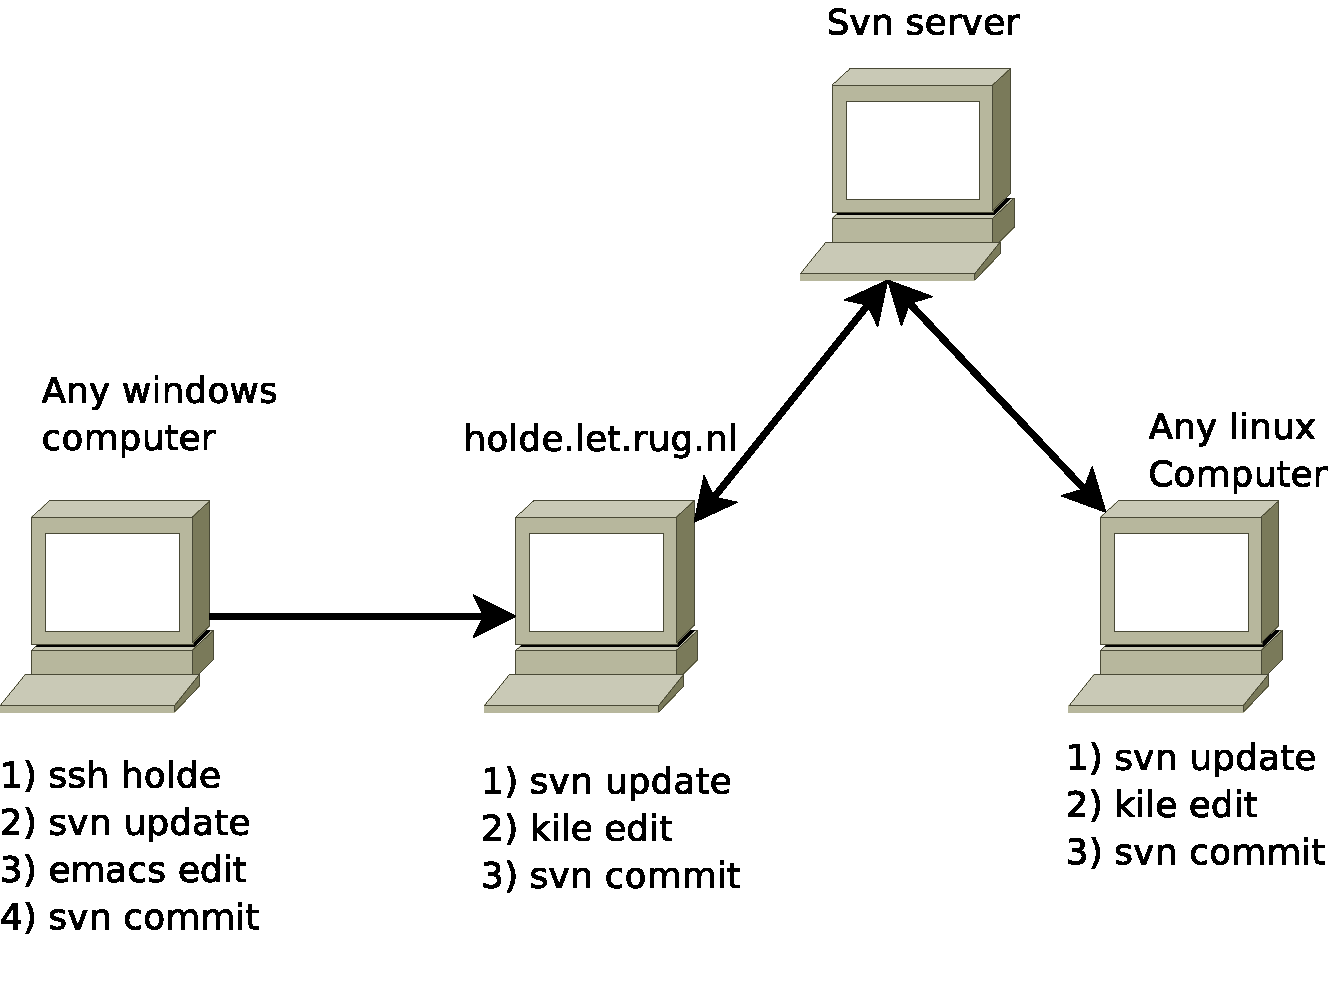
\includegraphics[scale=0.4]{pics/Doc_develop}
\captionof{figure}{How to work}
\label{how-to-work}
 % Doc_develop.eps: -11243639x-1 pixel, 300dpi, -95196.14x-0.01 cm, bb=0 0 639 481
\end{center}
\section*{Format of reading}
There is four kinds of format
	\begin{itemize}
	\item linux command looks like this: \linuxcommand{linux command}
	\item scree output looks like this:
	\begin{screen}
	 scree output
	\end{screen}
	\item options of command looks like: \op{option}
	\item hotkey looks like: \hotkey{hotkey}
	\item source code looks like:
	\begin{verbatim}
 		source code
	\end{verbatim}
	\end{itemize}

\ifx \allfiles \undefined
\end{CJK*}
\end{document}
\fi



\mainmatter
% !Mode:: "TeX:UTF-8:Soft"
\ifx \allfiles \undefined
\documentclass[a4paper,12pt,twoside]{book}
\usepackage{CJKutf8}
\usepackage[T1]{fontenc}
\usepackage{pifont}
\usepackage{graphicx}
\usepackage{capt-of}
\usepackage{color}
\newcommand{\linuxcommand}[1]{\texttt{\textcolor{blue}{\$ #1 \Pisymbol{psy}{191}}}}
\newcommand{\op}[1]{\textcolor{blue}{-#1}}
\newcommand{\hotkey}[1]{\framebox{#1}}
\newenvironment{screen}{\sffamily}{\rmfamily}

\begin{document}
\begin{CJK*}{UTF8}{song}
\title{命令}
\author{赵岩}
\date{}\maketitle

\else
\chapter{Command}
\fi

%you can check the page layout in the future, That is interesting thing to do it.
%\layout
\section{wild charcter}
介绍各种通配符的使用	
\begin{description}
	\item[Kind]:
	There are four kinds of wild character: *, ?, [ ],and \{\}.
	They are listed in the below table \vspace{2ex} \\
	\begin{center}
		\captionof{table}{wild character}
		\label{wild-character}
		\begin{tabular}{|c|c|}
		\hline Wildcard  & Matches \\
		\hline * & zero or more characters \\
		\hline ? & exactly one character \\
		\hline [abcde] & exactly one character listed \\
		\hline [a-e] & exactly one character in the given range \\
		\hline [!abcde] & any character that is not listed \\
		\hline [!a-e] & any character that is not in the given range \\
		\hline \{debian,linux\} & exactly one entire word in the options given \\
		\hline
		\end{tabular}
	\end{center}
	\item[Exmaple]:
		\begin{itemize}
		\item \linuxcommand{ls \{hd,sd\}[a-c]} will list all possible partitions.
		\item \linuxcommand{rm *[!abc] } delete any file doesn't end with a,b or c.
		\end{itemize}
	\item[Note]:
		\begin{itemize}
		\item \linuxcommand{cp *.*} will not copy all file, because some files don't have postfix name, that is a window habit.
		\item In order to avoid previous error, before you use wild characgter, you'd better use \linuxcommand{echo wildcharacter} to see whether they are what you want. It's a safer way, you need to follow it. all wild character is listed in Table \ref{wild-character} on page \pageref{wild-character}.
		\end{itemize}
	\end{description}
\section{redirection and pipes}
标准输出的代号为1,错误输出的代号为2. 你可以利用 \linuxcommand{command 1>stdout.txt 2>error.txt}来重新改变标准的输入输出设备。\linuxcommand{command 1>stdout.txt 2>\&1 }把错误输出重定以到标准输出上来。 \par

除了重定向命令以外,还有一个常用的技术就是管道。他可以把很多命令"粘贴"在一起,构成一个非常powerful的命令。例如:\linuxcommand{ls | less}就包含了一个管道。有的时候,管道后面的命令如果可以跟着两个参数,那么就有点麻烦。例如: \linuxcommand{ls -l |split -l 10 fileout} 我的本义是把ls的输出每10行一个,输出到fileout文件中去。但是这里有个问题,split命令会把fileout理解成输入。所以这里需要一个占位符。 我们可以写成\linuxcommand{ls -l | split -l 10 - fileout}。 这个小横杠就代表了标准输入了。如果一个命令需要多个参数的时候,好像都是可以使用这一招。例如paste命令。 \par

还有一点需要注意的就是,管道主要是处理的是文件的内容。而不是文件的名字。例如,你不能通过 \linuxcommand{ls *.txt | rm}来达到删除所有*.txt的目的。这是因为rm只关心文件的名字,而不关心文件的内容。为了解决这个问题,你可以通过 \linuxcommand{ls *.txt | xarg rm}
当然,管道后面的命令也有多个参数,如何指定到特殊的位置呢? 可以用\linuxcommand{ls *.txt | xarg -i cp {} /temp}。
\section{cp}
	\linuxcommand{cp }: copy files and directories
	\begin{description}
	\item[Options]: \\
	\begin{tabular}{c|p{0.82\textwidth}}
		\hline
		\op{a} & --archive same as -dpR \\
		\op{p} & same as --preserve=mode,ownership,timestamps \\
		\op{d} & --preserve=link, only copy link \\
		\hline
		\end{tabular}
	\item[Example]:
		\begin{itemize}
		\item \linuxcommand{cp -d a\_link c\_link}
		\end{itemize}
	\item[Note]:
		\begin{itemize}
		\item When you use cp without \op{p}, the target file mtime will be changed to current time.
		\end{itemize}
	\end{description}

\section{cd}
	\linuxcommand{cd directory}: go to a certain directory
	\begin{description}
	\item[Example]:
		\begin{itemize}
		\item \linuxcommand{cd -} exchange the previous two paths.
		\item \linuxcommand{cd \$HOME} go to \$HOME directory.
		\item \linuxcommand{(cd dir \&\& command)} go to some directory
			and commit a command, then return back original directory
			don't forget a pair of bracket.
		\item \linuxcommand{push . pop} will remember a directory, but you can't
			copy them across terminal.
		\item you can build a variable in shell WORK=$\sim$/project/\ldots{} , then you can
			\linuxcommand{cd \$WORK} directly.
		\item A better tool in linux is mc, you can use it to navigate your file system. It provides
			hotlist \hotkey{Ctrl+$\backslash$} and history \hotkey{Alt+Shit+h}. When you reach you target in the mc, \hotkey{Ctrl+o} can switch to terminal interface; you can use \hotkey{F2+1} get directory; \hotkey{F2+2} get file; \hotkey{F2+3} get all. in other terminal, use my linux command \linuxcommand{go} go to the target directory, and use
			mouse middle button to paste content to other X applictions.
		\end{itemize}
	\item[Note]:
		\begin{itemize}
		\item \linuxcommand{cd} is a embeded commmand.
		\item \linuxcommand{pwd} can tell you where you are.
		\end{itemize}
	\end{description}

\section{split}
	\linuxcommand{split [bl] file PREFIX}: split to make some smaller files
	\begin{description}
	\item[Options]: \\
		\begin{tabular}{c|p{0.82\textwidth}}
		\hline
		\op{l} & split according to lines. \\
		\op{b} & split according to size can be specified by b(byte), k(kilo) and m(mega).\\
		\hline
		\end{tabular}
	\item[Example]:
		\begin{itemize}
		\item \linuxcommand{ls -l / | split -l 10 - lsroot} in this command, you need to know the ``-'' meaning, it stands for the standerd input or output. (it need two fileanames as parameters :) )
		\item \linuxcommand{split -b 1.4m big small} it will produce files \emph{smallaa smallab smallac} \ldots. (it seems to support 26*26 possibilities.)
		\item \linuxcommand{cat small* >> big\_backup} combine all files back to original one.
		\end{itemize}
	\item[Note]:
		\begin{itemize}
		\item Just know it, I don't use it very often because the cheap price of storage device.
		\end{itemize}
	\end{description}

\section{touch}
	    \linuxcommand{touch [option] files}:
	    \begin{description}
	    \item[Options]:
		\begin{itemize}
		\item \op{t} you can use it to set file to anytime you want, detail can be found in man.
		\end{itemize}
	    \item[Example]:
		\begin{itemize}
		  \item \linuxcommand{touch file}
		\end{itemize}
	    \item[Note]:
		\begin{itemize}
		  \item There are three kind of times, \vspace{2ex} \\
		    \begin{tabular}{c|l}
		    \hline mtime & modification time\\
		    \hline ctime & status time such as permissoin and attribute; \\
		    \hline atime & last access time\\
		    \hline
		    \end{tabular} \vspace{2ex} \\
		    the touch file will set the mtime and atime to current time;
		  \item If you use this command to a exist file, all three time will be set to the current time.
		\end{itemize}
	    \end{description}

\section{ls}
	\linuxcommand{ls}: list content in a directory
	\begin{description}
	\item[Options]: \\
		\begin{tabular}{c|p{0.82\textwidth}}
		\hline
		\op{a} & list all hidden file.  \\
		\op{l} & detail list information. \\
		\op{t} & with \op{l}, sort by modification time.\\
		\op{r} & with \op{l}, reverse order.\\
		\op{h} & with \op{l}, show size with human readable format.\\
		\op{u} & with \op{lt}, will sort by atime; with -l, will give atime, sort by file name, just like \linuxcommand{ls -l --time=atime}\\
		\op{c} & the same as option \op{u}.\\
		\hline
		\end{tabular}
	\item[Example]:
		\begin{itemize}
		\item \linuxcommand{ls -ltr} will list all the lastest modification files
		\item \linuxcommand{ls -al} will give all the hiddent file
		\item \linuxcommand{ls -l --full-time} will give all detail time information.
		\item \linuxcommand{ls -d */} will only list directory, it is a little difficult to remember.
		\end{itemize}
	\item[Note]:
		\begin{itemize}
		\item Usually, we can use alias to build ll=ls -l command
		\item if you want to know size of every directory, \linuxcommand{du -csh * | sort}
		\end{itemize}
	\end{description}


\section{find}
	find is a little difficult, because the manual of this command can not be used in daily use. In the official document, you can see explaination below \linuxcommand{find [-H] [-L] [-P] [-D debugopts] [-Olevel] [path...] [expression]} you must pay attent to the [expression], The expression is made up of \emph{options} (which affect overall operation rather than  the  processing  of  a  specific file,  and  always  return true), \emph{tests} (which return a true or false value), and \emph{actions} (which have side effects and return a true or false value), all separated by \emph{operators}. In fact, It's comprised of bool expression in implementation, but only in some special use, you need to know the detail information of bool expression, such as \op{prune} example. I will explain it in the example section. \\
	I prefer to understand in this way: \linuxcommand{find where-to-look criteria what-to-do}:
	\begin{description}
	\item[Options in expression]: \\
		\begin{tabular}{c|p{0.82\textwidth}}
		\hline
		\op{maxdepth} & Descend at most levels (a non-negative integer) levels of directories.  \op{maxdepth 0}, only the current directory \\
		\op{mindepth} & Do not apply any tests or actions at levels less than levels (a non-negative integer). \op{-mindepth  1}  means process all files except the command line arguments. \\
		\op{depth} & depth first search \\
		other & other options can be found in manual of find. \\
		\hline
		\end{tabular}
	\item[Tests in expression]:
		\begin{itemize}
		\item \op{name}: find file according to name, support wild character (*, ?, []). See some explainations in example.
		\item \op{type}: find certain file type, \emph{d} diectory; \emph{f} regular file; \emph{l} link;
		\item \op{size n[cwbkMG]}: n can be +n(greater) ,-n(less) or n(equal). k(kilobyte) M(Megabyte) G(Gegabyte)
		\item \op{atime amin ctime cmin mtime mmin}: three kind of date and time. Detail can be found in \emph{touch} command;
		It support +n, n and -n number format.  \\
		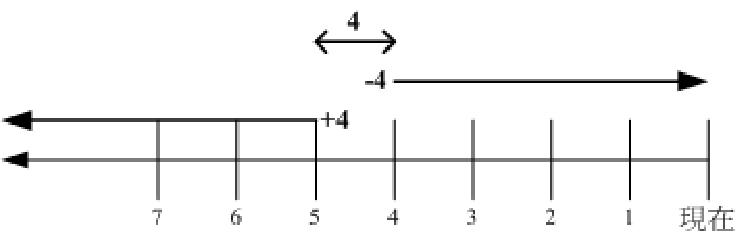
\includegraphics[scale=0.5]{pics/find_time}
		\item \op{user}: File is owned by user uname
		\item \op{group}: File belongs to group gname
		\item \op{perm}: File by permission. it support both symbolic(u+r) and number format(400). Just like time option, it also support n, -n and $\backslash$n(better format than +n). detail can be found in example.
		\item \op{path}: use when you want to exclude a directory	
		\end{itemize}
	\item[Actions in expression]:
		\begin{itemize}
		\item \op{print,print0,printf}: default actions is print
		\item \op{-exec }: execute some command
		\item \op{-prune}:
		\end{itemize}
	\item[Operators in expression]: \\
		\begin{tabular}{c|p{0.82\textwidth}}
		\hline
		() & Force  precedence \\
		! & no \\
		o & or \\
		, & both expr1 and expr2 are always evaluated \\
		\hline
		\end{tabular}
	\item[Example]:
		\begin{itemize}
		\item use of meta character \\
		\begin{tabular}{c|l}
		\hline \linuxcommand{find -name foo*bar} & shell will interpret * firstly(bad)\\
		\hline \linuxcommand{find -name foo$\backslash$*bar} & shell don't interpret *. \\
		\hline \linuxcommand{find -name ``foo*bar''} & the same as the previous  \\
		\hline \linuxcommand{find -name ``foo$\backslash$*bar''} & find exact file name. \\
		\hline
		\end{tabular}
		\item you also can use single quotes, but there is a different for shell
		\linuxcommand{find -name ``\$HOME''} will interpret it, but \linuxcommand{find -name '\$HOME'} will search it literaly. That's a very important difference bewteen them, you should know it.
		\item \linuxcommand{find /tmp /var/tmp . \$HOME -name foo 2>/dev/null} you can find in multi-directory and you can output error to /dev/null
		\item \linuxcommand{find / -mmin -10} learn which files got changed within 10 minnutes, it's also useful when you have download some file but can't locate it.(WATCH mmin, NOT mtime)
		\item \linuxcommand{find / -type f -mtime -7 | xargs tar -rf week\_add.tar} you can search files by two criteria. the default is \emph{and} relationship.
		\item \linuxcommand{find / -name /dev -prune | xargs tar \ldots} Normally, find returns the directory first, before any of the files in that directory.  This is useful when using the "-prune" action to prevent find from examining any files you want to ignore:
		\item \linuxcommand{find . -mmin +5 -mmin -10 } find files modifed between 6 and 9 minutes ago
		\item \linuxcommand{find . -maxdepth 1 -name '[!.]*' -printf 'Name: \%16f Size: \%6s$\backslash$n'} displays non-hidden (no leading dot) files in the current directory only (no subdirectories), with an custom output format:
		\item \linuxcommand{find . -type d | sort} get all directory and sort them.
		\item \linuxcommand{find /usr $\backslash$( -path /usr/sam1 -o -path /usr/sam2 $\backslash$) -prune -o -print} skip two directories when you conduct find.这个命令有点奇怪,我需要解释一下,prune通常只返回true,如果前面的path返回true,那么-o 后面的就没必要执行了,但是如果path返回false, 那么 path(false) and prune(true) 还是false.这个时候 -o后面的就得到执行的机会了。其实,find的各种应用形式,都是可以利用逻辑表达式的方式来理解的。当然,对于一些常用的应用,直接记住就可以了。
		\item \linuxcommand{find /    $\backslash$( -perm -4000 -fprintf /root/suid.txt '\%\#m \%u \%p$\backslash$n' $\backslash$) , $\backslash$ $\backslash$( -size +100M -fprintf /root/big.txt '\%-10s \%p$\backslash$n' $\backslash$)}  Traverse the filesystem just once, listing setuid files and directories into /root/suid.txt and large files into /root/big.txt.
		\end{itemize}
	\item[Note]:
		\begin{itemize}
		\item xargs is more efficent than -exec. 这是因为exec会把所有的参数传给后面的命令,如果参数过多,就会带来pararmter list is too long 这种错误。but it has two limitations. the first one is that not all commands accept the list of files at the end of the command, such as \linuxcommand{find -name $\backslash$*.txt | xargs cp /tmp} will not work. a solution is \linuxcommand{find -name $\backslash$*.txt | xargs -i cp \{\} /tmp}, to tell xargs use {} to replace the the result of find. Other solution is \linuxcommand{find -name $\backslash$*.txt | xargs cp -t /tmp}, and -t is an option scary for cp command. The other shortcoming is file name contain space. you can use \linuxcommand{find \ldots\ print0 | xargs -0 \ldots } to resolve this.
		\end{itemize}
	\end{description}
\section{grep}
	\linuxcommand{ grep [options] [-e PATTERN | -f FILE] [FILE...]}. you must specify files to search for, there is no default value. If it is empty, it will ask you to input something from standard input.
	\begin{description}
	\item[Options]: \\
		\begin{tabular}{c|p{0.82\textwidth}}
		\hline
		\op{i} & ignore case \\
		\op{v} & invert match\\
		\op{n} & show line name\\
		\op{w} & match the whole word, not substring \\
		\op{o} & only show match art, default show the match line\\
		\op{E} & support extend pattern\\
		\op{A, B, C} & after, before, context match.\\
		\hline
		\end{tabular}
	\item[PATTERN]:
		\begin{description}
		\item[Characters]: In fact, some grep don't support -P (perl options), you'd better avoid it. if you want to use ``* \^{} \$ [ ] \{ ( ) ? + '' literaly, you need to use $\backslash$ to escape it, or they have special meaning in the regular expression. dot stands for every character. if you want to match tab , you can use \hotkey{ctrl+v}, then tab to input a tab in a command line. below is common use characters.
		\begin{center}
			\begin{tabular}{|c|p{15em}|c|}
			\hline POSIX & Basic & perl \\
			\hline [[:alnum:]] & [0-9a-zA-Z] & $\backslash$w \\
			\hline [[:alpha:]] & [a-zA-Z] &  \\
			\hline [[:lower:]] & [a-z] &  \\
			\hline [[:upper:]] & [A-Z] &  \\
			\hline [[:digit:]] & [0-9] & $\backslash$d \\
			\hline [[:blank:]] & space and tab &  \\
			\hline [[:space:]] & more than blank, also include newline and carriage return &  \\
			\hline
			\end{tabular}
		\end{center}
	\item[Anchors]:
		\begin{itemize}
		\item \^{} begining of a line
		\item \op{\$} end of a line
		\item \op{$\backslash$< $\backslash$>}  begining of a word and end of a word. when you commit \linuxcommand{grep -E ``is$\backslash$>'' file} ``this's'' will be matched too.
		\end{itemize}
	\item[Alternations]:
		\begin{itemize}
		\item \op{|}: or, usually you put it within the a pair of ( ).
		\item \op{[]}: character set.
		\end{itemize}
	\item[Quantifiers]:
		\begin{itemize}
		\item \op{?} the preceding itme is optional and matched at most once
		\item \op{*} the preceding itme will be matched zero or moret times
		\item \op{+} the preceding itme will be matched one or moret times
		\item \op{\{n\}} the preceding itme will be matched exactly n times
		\item \op{\{n,\}} the preceding itme will be matched n or moret times
		\item \op{\{n,m\}} the preceding itme will be matched at least n times, but not moret than mtimes
		\end{itemize}
	\item[Grouping back references]:
		\begin{itemize}
		\item \op{()} group
		\item \op{$\backslash$num} back reference
		\end{itemize}
	\end{description}
	\item[Example]:
		\begin{itemize}
		\item \linuxcommand{grep -E ``love(rs|d)'' file} will match lovers and loved in file. you can't use [ ] to finish this task, because it only support single charater.
		\item \linuxcommand{grep -E ``$\backslash$([\^{}(]$\backslash$)''} to deal with this nest pairs, make sure that you can find the most inside
		\item \linuxcommand{grep ``EXIT\_'' /usr/include/*.h} You can search header files for particular definitions and
		function prototype.
		\item \linuxcommand{grep ``[]\^{} -]'' file} It's a little suprised, if you want to find ``] \^{} -'' you can put ]
		the first postion, put - the last postoin, and \^{}  everwhere but first position. in this way , you don't need escape them
		\item \linuxcommand{grep -c `date +\%b`} place a command inside a pair of backward marks
		\item \linuxcommand{grep 'a|b' file} doesn't work as your respect, you should use \linuxcommand{grep -E 'a|b' file}. you can see differences in Note.
		\end{itemize}
	\item[Note]:
		\begin{itemize}
		\item differences between grep and grep -E and egrep can be found in table ,
		you can concluded that best tool seem to be the \linuxcommand{grep -E} \\
		\begin{center}
 			\begin{tabular}{|c|c|c|}
			\hline grep & grep -E & egrep \\
			\hline $\backslash$+ & + or & yes \\
			\hline $\backslash$? & ? &  yes \\
			\hline ex1 $\backslash$| e2 & e1 | e2 & yes \\
			\hline $\backslash$(ex$\backslash$) & (ex) & yes \\
			\hline $\backslash${m,n$\backslash$} & {m,n} & no \\
			\hline no & $\backslash$w & $\backslash$w \\
			\hline no & $\backslash$< $\backslash$> & $\backslash$< $\backslash$> \\
			\hline
			\end{tabular}
		\end{center}
		\item Anyway, use -E is good habit. It can save your typing in the future.:)
		\end{itemize}
	\end{description}
\section{gzip}
	\begin{description}
	\item[Options]: \\
		\begin{tabular}{c|p{0.82\textwidth}}
		\hline
		\op{c} & output to screen, \\
		\op{d} & decompress \\
		\op{v} & verbose\\
		\op{r} & recursive directory, it will compress all files under this directory individually. \\
		\hline
		\end{tabular}
	\item[Example]:
		\begin{itemize}
		\item \linuxcommand{gzip -c file >file1.gz} By default, gzip will delete file and produce a file.gz. if you
		want to keep origanl one, you can use -c option like this example.
		\item \linuxcommand{gzip -d file1.gz}, it will produce file1 and delete file1.gz
		\end{itemize}
	\item[Note]:
		\begin{itemize}
		\item  by default, gzip will delete origal file, you don't need give it target file name.(it add .gz when compress or delete .gz when decompress
		\item \linuxcommand{zless} and \linuxcommand{zcat} to view the compress text file directly.
		\end{itemize}
	\end{description}
\section{bzip2}
	\begin{description}
	\item[Options]: \\
		\begin{tabular}{c|p{0.82\textwidth}}
		\hline
		\op{k} & keep original file, \\
		\op{1,\ldots 9} & level of compression. better compression, slower.\\
		\hline
		\end{tabular}
	\item[Example]:
		\begin{itemize}
		\item the options just like gzip, you can take a look at gzip command examples.
		\end{itemize}
	\item[Note]:
		\begin{itemize}
		\item  Compared with gzip, it don't support -r options, and other option is the same.
		\item \linuxcommand{bzless} and \linuxcommand{bzcat} to view the compress text file directly.
		\item In compression rate, the bzip2 is better than gzip. 文件名的后缀通常为bz2或者bz。如果是包文件,也可能是tbz2
		\end{itemize}
	\end{description}
\section{tar}
	\begin{description}
	\item[Options]:\\
		\begin{tabular}{c|p{0.82\textwidth}}
		\hline
		\op{p} & same permisstion \\
		\op{C} & extract to different directory \\
		\hline
		\end{tabular} \vspace{1ex} \\
		
		\begin{tabular}{|c|c|c|}
		\hline j(bzip2) & c(create) &   \\ \cline{2-2}
			& t(check) & v(verbose) \\ \cline{2-2}
			z(gzip)  & x(extract) &   \\
		\hline
		\end{tabular}
	\item[Example]:
		\begin{itemize}
		\item \linuxcommand{tar -xv -f file.tar} to extract file for tar ball
		\item \linuxcommand{tar -cv -f file.tar dirName} to create a tar ball contain the whole dirName
		\item \linuxcommand{tar -jxv -f file.tbz2 -C /tmp} to extract and unzip a tar ball and copy it the /tmp
		\end{itemize}
	\item[Note]:
		\begin{itemize}
		\item  You'd better use -f to specify tar.gz name seperately. It's more obvious.
		\end{itemize}
	\end{description}
\section{file}
	\begin{description}
	\item[Options]: \\
		\begin{tabular}{c|p{0.82\textwidth}}
		\hline
		\op{s} & read special file \\
		\hline
		\end{tabular}
	\item[Example]:
		\begin{itemize}
		\item \linuxcommand{sudo file -s /dev/hda1} you can use -s optoin, and you also need root permission.
		\end{itemize}
	\item[Note]:
		\begin{itemize}
		\item  usually, file name doesn't have extension, use file to know what type it is. linux系统文件通常没有后缀名,所以你最好用file命令先判断一下这个文件是个什么类型的文件。
		\end{itemize}
	\end{description}
\section{locate}
	\begin{description}
	\item[Options]: \\
		\begin{tabular}{c|p{0.82\textwidth}}
		\hline
		\op{w} & default, whole name\\
		\op{b} & Results are considered to match if the pattern specified matches the final component of the name of a file as listed  in the database.  This final component is usually referred to as the `base name'. \\
		\hline
		\end{tabular}
		
	\item[Example]:
		\begin{itemize}
		\item \linuxcommand{locate linux.tex} will output linux.tex and linux.tex.backup
		\item \linuxcommand{locate -b ``$\backslash$linux.tex''} will only output linux.tex
		\end{itemize}
	\item[Note]:
		\begin{itemize}
		\item  locate search file in a database file. \linuxcommand{updatedb} to update this database
		\end{itemize}
	\end{description}
\section{which}
	\begin{description}
	\item[Options]: \\
		\begin{tabular}{c|p{0.82\textwidth}}
		\hline
		 \op{a} & print all matching pathname\\
		\hline
		\end{tabular}
	\item[Example]:
		\begin{itemize}
		\item \linuxcommand{which ls}
		\end{itemize}
	\item[Note]:
		\begin{itemize}
		\item  only located command, you can use \linuxcommand{find} for ordinary file.
		\end{itemize}
	\end{description}
\section{whereis}
	locate binary, source and manual of file(command)
	\begin{description}
	\item[Options]:\\
		\begin{tabular}{c|p{0.82\textwidth}}
		\hline
		 \op{empty} & empty\\
		\hline
		\end{tabular}
	\item[Example]:
		\begin{itemize}
		\item \linuxcommand{whereis man} output is
		\begin{screen}
		/usr/bin/man /usr/local/man /usr/share/man /usr/share/man/man1/man.1.gz  /usr/share/man/man7/man.7.gz
		\end{screen}
		there are two different kind of manual page for man, you can use \linuxcommand{man 1 man} and \linuxcommand{man 7 man } to read them. Meanings of number can be found in man 1 man.
		\end{itemize}
	\item[Note]:
		\begin{itemize}
		\item  it seems that it commonly used for command and not for ordinary file, just like which.
		\end{itemize}
	\end{description}
\section{ps}
	process status report a snapshot of the current processes
	\begin{description}
	\item[Options]: \\
		\begin{tabular}{c|p{0.82\textwidth}}
		\hline
		 \op{a} & select all process except session leader(?)\\
		\hline
		\end{tabular}
	\item[Example]:
		\begin{itemize}
		\item \linuxcommand{ps -ux} list current user process
		\item \linuxcommand{ps -aux | grep 'name' }
		\end{itemize}
	\item[Note]:
		\begin{itemize}
		\item  you can find STAT code in by \linuxcommand{man ps}
		\end{itemize}
	\end{description}
\section{kill}
	send a singal to a process
	\begin{description}
	\item[Options]: \\
		\begin{tabular}{c|p{0.82\textwidth}}
		\hline
		\op{l} & list all aviable singal.\\
		\hline
		\end{tabular}
		
	\item[Example]:
		\begin{itemize}
		\item \linuxcommand{kill -9 -1} kill all processes you can kill
		\item \linuxcommand{kill 123} send SIGTERM to pid 123,
		\end{itemize}
	\item[Note]:
		\begin{itemize}
		\item  you should use \linuxcommand{ps} to find pid value.
		\item  -9 means kill, This will not be blocked by the application.
		\end{itemize}
	\end{description}
\section{jobs}
	list the jobs you are runing in the backgroud and foreground
	\begin{description}
	\item[Options]:\\
		\begin{tabular}{c|p{0.82\textwidth}}
		\hline
		 \op{empty} & empty\\
		\hline
		\end{tabular}
	\item[Example]:
		\begin{itemize}
		\item
		\end{itemize}
	\item[Note]:
		\begin{itemize}
		\item it will output job num,usually use before \linuxcommand{fg jobnum}and \linuxcommand{ bg jobnum}to
		\item you can ues \linuxcommand{command \&} to put it to background \emph{running}, When you use Ctrl+Z,
		it just put the current processing to background \emph{suspending}, then you can use bg to change it to
		background \emph{running}. \linuxcommand{fg jobnum} can put it ot foreground running, at this time, you
		can use Ctrl+C to stop it. Or use kill in other terminal console.
		\end{itemize}
	\end{description}
\section{wc}
	word count, print line, word, and byte count of a file
	\begin{description}
	\item[Options]: \\
		\begin{tabular}{c|p{0.82\textwidth}}
		\hline
		\op{l} & only print line number \\
		\op{w} & only print word number\\
		\op{m} & only print character number\\
		\op{L} & print the longest line\\
		\hline
		\end{tabular}
	\item[Example]:
		\begin{itemize}
		\item \linuxcommand{wc -l file}
		\end{itemize}
	\item[Note]:
		\begin{itemize}
		\item  \op{L} is very interesting option
		\end{itemize}
	\end{description}	

\section{history}
	list all commands you have typed.
	\begin{description}
	\item[Options]: \\
		\begin{tabular}{c|p{0.82\textwidth}}
		\hline
		\hline
		\end{tabular}
	\item[Example]:
		\begin{itemize}
		\item \linuxcommand{history | grep command1} to search a command in a long history list.
		\end{itemize}
	\item[Note]:
		\begin{itemize}
		\item
		\end{itemize}
	\end{description}	

\section{lp}
	print a document
	\begin{description}
	\item[Options]: \\
		\begin{tabular*}{0.9\textwidth}{c|l}
		\hline
		\op{sides=two-sided-long-edge} & two sides print\\
		\hline
		\end{tabular*}
	\item[Example]:
		\begin{itemize}
		\item \linuxcommand{fmt a.txt |pr| lp} fmt is simple command, just create a longer praragraph. And pr maybe can add page number to the page
		\end{itemize}
	\item[Note]:
		\begin{itemize}
		\item  It seems that lp is better than lpr because it is more compatiable.
		\end{itemize}
	\end{description}
\section{sort}
	sort lines of text file
	\begin{description}
	\item[Options]:\\
		\begin{tabular}{c|p{0.82\textwidth}}
		\hline
		\op{f} & make all lines uppercase before sorting \\
		\op{d} & --dictionary-order\\
		\op{f} & --ignore-case\\
		\op{n} & --numeric-sort\\
		\op{r} & --reverse the result of comparisons\\
		\op{+m} & start at the first character of m+1th fiedl\\
		\op{-n} & end at the last character of the nth field\\
		\op{tx} & use x as the field delimiter\\
		\hline
		\end{tabular}
	\item[Example]:
		\begin{itemize}
		\item \linuxcommand{sort -r +2 -3 company.data}
		\item \linuxcommand{sort -t: +1 -2 company.data}
		\end{itemize}
	\item[Note]:
		\begin{itemize}
		\item It's often used in pipe
		\item You also can sort according to two columns
		\end{itemize}
	\end{description}
\section{less}
	\begin{description}
	\item[Options]: \\
		\begin{tabular}{c|p{0.82\textwidth}}
		\hline
		\op{N} & print line number \\
		\hline
		\end{tabular}
	\item[Example]:
		\begin{itemize}
		\item \linuxcommand{file1 file2 file3} you can use :n :q to navigate these files
		\item you can use v command to open your default editor in less
		\item :e to open a new document, :d to delete the current one
		\end{itemize}
	\item[Note]:
		\begin{itemize}
		\item It's more like only read editor, you should use different commands to control it.
		\item if you forget some commands usage, you can use command h .
		\end{itemize}
	\end{description}
\section{uniq}
	report or omit repeated lines
	\begin{description}
	\item[Options]: \\
		\begin{tabular}{c|p{0.82\textwidth}}
		\hline
		\op{c} & prefix lines by the number of occurrences \\
		\hline
		\end{tabular}
	\item[Example]:
		\begin{itemize}
		\item \linuxcommand{sort file | uniq -c } give you unigram information
		\end{itemize}
	\item[Note]:
		\begin{itemize}
		\item It must be used in a sorted file
		\end{itemize}
	\end{description}
\section{xxd}
	make a hexdump or do the reverse
	\begin{description}
	\item[Options]:\\
		\begin{tabular}{c|p{0.82\textwidth}}
		\hline
		\op{b} & switch to bits(binary digits) dump \\
		\op{c cols} & format cols octets per line\\
		\op{l len} & stop after writing len octets\\
		\hline
		\end{tabular}
	\item[Example]:
		\begin{itemize}
		\item \linuxcommand{xxd -l 120 -c 12 xxd.1}
		\end{itemize}
	\item[Note]:
		\begin{itemize}
		\item a similar command is like \linuxcommand{od -t x1}, default output of od
		is based on octal, the output is little strange, because it divived binary bit every three bits, for exmaple 00100000 00100000 od -t o1 will outupt 040 040, and od -t o2 will output 020040 (0,010,000,0 00,100,000). Do you still understand it:)
		\end{itemize}
	\end{description}
\section{cut}
	remove sections from each line of a file
	\begin{description}
	\item[Options]: \\
		\begin{tabular}{c|p{0.82\textwidth}}
		\hline
		\op{d} & field delimiter \\
		\op{f} & for field \\
		\op{c} & field delimiter is character\\
		\hline
		\end{tabular}
	\item[Example]:
		\begin{itemize}
		\item \linuxcommand{cut -d``*'' -f 2-3} will output B*C. it will not change the original content, only cut part of out
		\end{itemize}
	\item[Note]:
		\begin{itemize}
		\item If you need change format from the inputfile, \linuxcommand{awk} or \linuxcommand{sed } is two better choices.
		\end{itemize}
	\end{description}
\section{type}
	\linuxcommand{type }: Using the "type" command shows how any of the commands or names you include beyond the command would be interpreted if input. This means that it would explain any macros you created, any commands you've aliased or any other additions you've made to the BASH
	\begin{description}
	\item[Options]: \\
		\begin{tabular}{c|p{0.82\textwidth}}
		\hline
		\op{a} Using "-a" will display a list of all executables with the file name.
		\op{t} Using "-t" will display a single word relating to the actual type of the command you wish to describe (alias, function, builtin, keyword or file).
		\op{p} Using "-p" will display the name of the file used with the "type" command.
		\end{tabular}
	\item[Example]:
		\begin{itemize}
		\item empty
		\end{itemize}
	\item[Note]:
		\begin{itemize}
		\item it's a little like \linuxcommand{whereis}
		\end{itemize}
	\end{description}

\section{tr}
	translate or delete characters
	\linuxcommand{tr [option] \ldots SET1 [SET2]}
	\begin{description}
	\item[Options]: \\
		\begin{tabular}{c|p{0.82\textwidth}}
		\hline
		\op{c} & --complement \\
		\op{d} & --delete\\
		\op{s} & --squeeze-repeats\\
		\op{t} & --truncate-set1, may be used only when translating.
		Interpreted sequences are $\backslash$NNN, $\backslash$b backspace, $\backslash$n new line $\backslash$r return, $\backslash$t horizontal tab, $\backslash$v vertical tab. It also can contain [:alnum:] [:digit:] \\
		\hline
		\end{tabular}
	\item[Example]:
		\begin{itemize}
		\item \linuxcommand{tr A-z a-z <a.txt | tr -d ``.,?''|tr -s ' ' '$\backslash$012'|sort|unqi -c} this command will
		produce a unigram for a text file.
		\end{itemize}
	\item[Note]:
		\begin{itemize}
		\item It mainly applied in character level.
		\item It doesn't include file name argument, you should use <file.name to redirect.
		\end{itemize}
	\end{description}
\section{join}
	join lines of two files on a common field
	\begin{description}
	\item[Options]: \\
		\begin{tabular}{c|p{0.82\textwidth}}
		\hline
		\op{t} & delimiter character \\
		\op{i} & ignore case \\
		\op{1 num} & use this num to specify field in the first file \\
		\op{2 num} & use this num to specify field in the second file \\
		\hline
		\end{tabular}		
	\item[Example]:
		\begin{itemize}
		\item
		\begin{screen}
		==> /etc/passwd <==  \\
		root:x:0:0:root:/root:/bin/bash \\
		bin:x:1:1:bin:/bin:/sbin/nologin \\
		daemon:x:2:2:daemon:/sbin:/sbin/nologin \\

		==> /etc/group <== \\
		root:x:0:root \\
		bin:x:1:root,bin,daemon \\
		daemon:x:2:root,bin,daemon \\
		\end{screen}
		
		\linuxcommand{join -t ':' -1 4 /etc/passwd -2 3 /etc/group}
		will produce output like this \\

		\begin{screen}
		0:root:x:0:root:/root:/bin/bash:\textit{root:x:root} \\
		 1:bin:x:1:bin:/bin:/sbin/nologin:\textit{bin:x:root,bin,daemon} \\
		 2:daemon:x:2:daemon:/sbin:/sbin/nologin:\textit{daemon:x:root,bin,daemon} \\
		\end{screen}
		\end{itemize}
	\item[Note]:
		\begin{itemize}
		\item
		\end{itemize}
	\end{description}
\section{du}
	estimate file space usage
	\linuxcommand{tr [option] \ldots SET1 [SET2]}
	\begin{description}
	\item[Options]: \\
		\begin{tabular}{c|p{0.82\textwidth}}
		\hline
		\op{c} & --total, produce a grand total \\
		\op{h} & --human-readable\\
		\op{s} & --summarize, display only a total for each argument\\
		\hline
		\end{tabular}	
	\item[Example]:
		\begin{itemize}
		\item \linuxcommand{du -sch *} this command will
		print all directory size
		\item \linuxcommand{du -sh *} will print all leaf directory
		size
		\end{itemize}
	\item[Note]:
		\begin{itemize}
		\item you must give a directory name or * as a argument.
		\end{itemize}
	\end{description}
\section{dos2unix}
	Converts text files between DOS and Unix formats.
	\begin{description}
	\item[Options]: \\
		\begin{tabular}{c|p{0.82\textwidth}}
		\hline
		\op{empty} & empty \\
		\hline
		\end{tabular}
	\item[Example]:
		\begin{itemize}
		\item \linuxcommand{dos2unix file} this command will change return format.
		\end{itemize}
	\item[Note]:
		\begin{itemize}
		\item \linuxcommand{unix2dos} does the reverse thing
		\item it will overwrite the input file directly
		\end{itemize}
	\end{description}
\section{tail}
	output the last part of files
	\begin{description}
	\item[Options]: \\
		\begin{tabular}{c|p{0.82\textwidth}}
		\hline
		\op{n} & --lines=N output the last N lines, instead of the last 10 \\
		\op{f} & --follow, output appended data as the file grows \\
		\hline
		\end{tabular}
	\item[Example]:
		\begin{itemize}
		\item \linuxcommand{tail -f log} this command will monitor the log file
		\end{itemize}
	\item[Note]:
		\begin{itemize}
		\item empty
		\end{itemize}
	\end{description}
\section{ldd}
	print shared library dependencies
	\begin{description}
	\item[Options]: \\
		\begin{tabular}{c|p{0.82\textwidth}}
		\hline
		\op{empty} & empty \\
		\hline
		\end{tabular}
	\item[Example]:
		\begin{itemize}
		\item \linuxcommand{ldd $\backslash$bin$\backslash$ls}
		\end{itemize}
	\item[Note]:
		\begin{itemize}
		\item empty
		\end{itemize}
	\end{description}
\section{lpq}
	show printer queue status
	\begin{description}
	\item[Options]: \\
		\begin{tabular}{c|p{0.82\textwidth}}
		\hline
		\op{empty} & empty \\
		\hline
		\end{tabular}
	\item[Example]:
		\begin{itemize}
		\item \linuxcommand{lpq}
		\end{itemize}
	\item[Note]:
		\begin{itemize}
		\item \linuxcommand{lprm} to delete a print task
		\item \linuxcommand{lp} to print a document
		\end{itemize}
	\end{description}
\section{free}
	Display amount of free and used memeory in the sytem
	\begin{description}
	\item[Options]: \\
		\begin{tabular}{c|p{0.82\textwidth}}
		\hline
		\op{b} & dispaly in byte, and you can think there are other options, k,m,g \\
		\hline
		\end{tabular}
	\item[Example]:
		\begin{itemize}
		\item \linuxcommand{free -m}
		\end{itemize}
	\item[Note]:
		\begin{itemize}
		\item
		\end{itemize}
	\end{description}
\section{netstat}
	Print network connections, routing tables.
	\begin{description}
	\item[Options]: \\
		\begin{tabular}{c|p{0.82\textwidth}}
		\hline
		\op{empty} & empty\\
		\hline
		\end{tabular}
	\item[Example]:
		\begin{itemize}
		\item \linuxcommand{netstat -m}
		\end{itemize}
	\item[Note]:
		\begin{itemize}
		\item \op{a} and \op{n} are used more often.
		\end{itemize}
	\end{description}
\section{nl}
	number lines of files
	\begin{description}
	\item[Options]: \\
		\begin{tabular}{c|p{0.82\textwidth}}
		\hline
		\op{empty} & empty\\
		\hline
		\end{tabular}
	\item[Example]:
		\begin{itemize}
		\item
		\end{itemize}
	\item[Note]:
		\begin{itemize}
		\item  you can use less -N to get the same result, but here, it support some logical page which inlcudes header, body and footer
			The beginnings of the sections of logical pages are indicated in the input file by a line containing nothing except one of the following delimiter strings:
			$\backslash$:$\backslash$:$\backslash$: start of header \\
			$\backslash$:$\backslash$: start of body \\
			$\backslash$: start of footer \\
		\end{itemize}
	\end{description}
\section{diff}
	Display amount of free and used memeory in the sytem
	\begin{description}
	\item[Options]:\\
		\begin{tabular*}{0.9\textwidth}{c|l}
		\hline
		\op{y} & Display two columns \\
		\op{--suppress-common-lines} & Do not output common lines \\
		\hline
		\end{tabular*}
	\item[Example]:
		\begin{itemize}
		\item
		\end{itemize}
	\item[Note]:
		\begin{itemize}
		\item \linuxcommand{diff new.log old.log | grep \^{} $\backslash$< | wc -l} find how  many difference.
		\end{itemize}
	\end{description}	
\section{df}
	report filesystem disk space usage
	\begin{description}
	\item[Options]: \\
		\begin{tabular}{c|p{0.82\textwidth}}
		\hline
		\op{h} & dispaly human-readable\\
		\hline
		\end{tabular}
	\item[Example]:
		\begin{itemize}
		\item \linuxcommand{df -h}
		\end{itemize}
	\item[Note]:
		\begin{itemize}
		\item It is a little different with du, and du is used more often.
		\end{itemize}
	\end{description}
\section{pdftops}
	pdftops - Portable Document Format (PDF) to PostScript converter (version 3.00)
	\begin{description}
	\item[Options]:\\
		\begin{tabular}{c|p{0.82\textwidth}}
		\hline
		\op{eps} & produce eps picture\\
		\hline
		\end{tabular}
	\item[Example]:
		\begin{itemize}
		\item \linuxcommand{pdftops -eps file.pdf file.eps}
		\end{itemize}
	\item[Note]:
		\begin{itemize}
		\item First, you can use printer to print visio to pdf, than use this command to change
		it to eps, and \LaTeX\ support eps. that is good.
		\end{itemize}
	\end{description}
\section{wget}
	non-interactive network downloader.
	\begin{description}
	\item[Options]:\\
		\begin{tabular}{c|p{0.82\textwidth}}
		\hline
		\op{empty} & empty \\
		\hline
		\end{tabular}
	\item[Example]:
		\begin{itemize}
		\item \linuxcommand{wget -r -np -nd --accept=iso http://example.com/i386/} 其中,-np 的作用是不遍历父目录,-nd 表示不在本机重新创建目录结构。--accept=iso 选项,这指示 wget 仅下载 i386 目录中所有扩展名为 iso 的文件。你也可以指定多个扩展名,只需用逗号分隔即可。
		\end{itemize}
	\item[Note]:
		\begin{itemize}
		\item
		\end{itemize}
	\end{description}

\chapter{Application}
\section{Ubuntu}
		\begin{itemize}
		\item Nautilus start typing the search term. A small search text field will appear near the bottom-right of the window and files/folders will be matched as you type
		\item unrar  filename.rar, replacing filename.rar with that which you downloaded
		\item Click System ->Administration-> Software Sources. Click the Download from dropdown list and then select Other. In the list of servers, choose any you wish. You'll need to reload the package lists from the server when prompted.
		\item If Windows didn't cleanly shutdown then Ubuntu will refuse to mount the partition. If, even after Windows is cleanly shutdown, the Windows partition refuses to appear, then run a chkdsk on the partition from within Windows.
		\item Terminal click Edit -> Current Profile and select the Colors tab. Then remove the check from Use colors from system theme and select a replacement from the Built-in schemes dropdown list. Try the Green on Black scheme.
		\item Alt + F2 . Then type the name of the program. If it needs to run with root privileges, just type gksu beforehand.
		\item If Windows is refusing to boot, for whatever reason, you can try repairingthe file system from within Ubuntu. Use Synaptic to search for the ntfsprogs package. Once it's installed, unmount your Windows partition (if it's mounted) and
		type sudo ntfsfix /dev/sda1 to check and fix the partition (assuming your Windows partition is /dev/sda1. likely if you installed Ubuntu in a dual-boot configuration on a computer already running Windows).
		\item The following will send everything currently on the current screen (command-line prompts included) to a text file called output.txt:\$ sudo screendump > output.txt
		The command has to be issued as root because of permission issues but the resulting file will be owned by you.
		\item 	If you're working on a virtual console and want to kill the GUI for any reason, typing the following will kill GNOME Display Manager (gdm), which ``owns'' the desktop processes:
		\linuxcommand{sudo killall gdm}. To get the GUI back following this, start gdm again: \linuxcommand{sudo gdm}
		\item do the following:open a terminal window and type \linuxcommand{cat /etc/lsb-release}. You can also click Help ! About Ubuntu to check version
		\item click System->Preferences->Keyboard Shortcuts and look in the list for Run a Terminal, which will be under the Desktop heading. Click the word Disabled alongside it, and then hit Ctrl + Alt + t .
		\item Start Firefox and, in the address line, type about:plugins. The headings show the type of content the plugin is designed to pick-up and below is listed the Ubuntu plugin that handles the content.
		\item To check virus, To install ClamTK and also ClamAV, use Synaptic to search for the clamtk package.
		\item To quickly view a picture from the command line, just type \linuxcommand{eog filename}.
		\item To move any unmaximized window around, hold down Alt and then click and drag anywhere in the window.
		\item There are a number of ways of converting a text file into a PDF at the command line. Perhaps easiest is to ``print'' it to Ubuntu's PDF printer driver. The file will then be saved to the PDF folder in your /home folder. This tip uses the lp command, telling it which printer to use with the options \op{d} : \linuxcommand{lp -d PDF textfile.txt}
		\item Uninstall Ubuntu can be seen in ubuntu\_kung\_fu tip 118
		\item \linuxcommand{sudo mkdir /media/ISO }, \linuxcommand{sudo mount -o loop ~/ubuntu.iso /media/ISO}
		Note that the first command creates a mount point and doesn't need to be typed in future. Once the ISO image is mounted, an icon for it will automatically appear on the desktop.To unmount the image, type sudo umount /media/ISO in the terminal window.
		\item To clear the cache from the command-line, type the following: \linuxcommand{sudo apt-get clean}
		\item use the pdftotext program: pdftotext filename.pdf. This will create a .txt file containing the contents of the PDF. To view it, use the less command: less filename.txt. To extract the images from the PDF, use the pdfimages command. You'll need to specify the filenames for the pictures, and also the -j command option to ensure the photographic images are outputted as JPEG. For example, the following: \linuxcommand{pdfimages -j filename-pdf pictures}
		\item Start your favorite application, highlight the mouse cursor over the menu option you want to change, and hit the new
		combination. You'll see that the menu instantly reflects the changes. To remove any keyboard shortcut, just hit the Backspace key
		(not the Delete key?that will cause Delete to be the new shortcut).
		\item Just use Synaptic to install nautilus-open-terminal. Then log out and back in again. In future you can either right-click blank
		space in a particular folder and select Open in terminal to open a terminal window automatically in that folder
		% \item Now run it through the column command by piping the output of the previous command, as follows: \$ cat /etc/fstab|column ?t
		\item \$ xclip < /etc/fstab
		...which will add the contents of the /etc/fstab configuration file to the clipboard, or you can pipe the output of a command into it:
		\linuxcommand{dmesg|xclip}
		...which will place the output of the dmesg command in the clipboard (dmesg shows system log output, and can be useful when diagnosing problems).
	\end{itemize}

\section{KDE}
		\begin{itemize}
		\item Konqueror F9 will show or hide Navigation Panel! F4 will open shell window. I mainly use mc now.
		\item in Konsole, you can press shift+-> to jump to another Shell window, it's convenient for you to finish some tasks
		\end{itemize}

\ifx \allfiles \undefined
\end{CJK*}
\end{document}
\fi	

% !Mode:: "TeX:UTF-8:Soft"
\ifx \allfiles \undefined
\documentclass[a4paper,12pt,twoside]{book}
\usepackage{CJKutf8}
\usepackage[T1]{fontenc}
\usepackage{pifont}
\usepackage{graphicx}
\usepackage{capt-of}
\usepackage{color}
\newcommand{\linuxcommand}[1]{\texttt{\textcolor{blue}{\$ #1 \Pisymbol{psy}{191}}}}
\newcommand{\op}[1]{\textcolor{blue}{-#1}}
\newcommand{\hotkey}[1]{\framebox{#1}}
\newenvironment{screen}{\sffamily}{\rmfamily}

\begin{document}
\begin{CJK*}{UTF8}{song}
\title{工具}
\author{赵岩}
\date{}\maketitle

\else
\chapter{Tools}
\fi
\section{mac}
四个基本原则:
\begin{itemize}
\item 严格控制时间
\item 任务驱动
\item 随时文档化
\item 学以致用(要不很容易就忘了)
\end{itemize}
常用快捷键,能够减少鼠标的使用。command就是window键。
ctrl+a,e跳到行头或行尾。
command + ~ 可以在不同的文档中切换。command+ tab可以在不同的程序中切换。
quicksiver 可以随时打开,关闭程序,如果一个程序当前active,你可以cmd+w,如果一个程序不可见,用quicksiver。
firework中, ctrl+T可以切换所有的tab。command+~切换不同的窗口。cmd+left arrow, right arrow, 切换历史纪录
cmd+L切换到地址栏。
\section{win7}
\begin{itemize}
\item win+arrow key can dock windows to left,right,maximize and minimize, that is very useful
\item win+p can control project camera
\item win+1,2,3 can launch programme in task bar quickly
\item when the explore becomes slowly, you should check tool--manager add-ons to see which add-on is slow.
\item right mouse key can produce a jump list, the content of jump list will change according to the type of progamme.
\item move windows to the left side can change it to 50\% width.
\item win+L to lock the windows
\end{itemize}

\subsection{iexplore}
\begin{itemize}
\item learn to use tab to explore the internet. that is very useful, don't try to open a new page in a new windows, but in a new tab. \hotkey{ctrl+num} to navigate the tabs. and \hotkey{ctrl+click} to open a link in a new tab. \hotkey{ctrl+T} open a new tab. \hotkey{ctrl+w} to close the current tab.
\end{itemize}



\section{主要使用软件}
\begin{tabular}{|c|c|c|c|}
\hline & mac & windows & linux  \\
\hline diagramming & \parbox[c]{10em}{\centering OmniGraff \\ ConceptDraw}& visio & Dia   inkscape \\
\hline vector drawing & illustrator & coreldraw illustrator & ? \\
\hline edit & textmate & Ultraedit & Emacs \\
\hline doc & mactex & Ctex & livetext \\
\hline web & dreamweaver & dreamweaver & ? \\
\hline screenshot & jing snapZ pro & snagit & ? \\
\hline screencast & \parbox[c]{10em}{\centering screen flow \\ camtasia }& camtasia & Xvidcap \\
\hline download & amule 或 Vuze & emule & amule  \\
\hline audio editor & \parbox[c]{10em}{\centering audacity(业余) \\ logic(专业)} & \parbox[c]{10em}{\centering gold wave(业余)\\ adobe audition(专业)} & ? \\
\hline video editor & \parbox[c]{10em}{\centering finalcut \\  imoive(业余)} & \parbox[c]{10em}{\centering premiere(专业) \\ 会声会影 (业余)}& ? \\
\hline

\end{tabular}
	
\section{commander}
\subsection{total commander}
\begin{itemize}
\item to jump to the folder as quick as possible, \hotkey{atl+down arrow} to show history folder. \hotkey{ctrl+D} to show the favorite folder. \hotkey{alt+f1,f2} to change left and right drivers. \hotkey{ctrl+s} to open a search bar , you can input a letter.

\item \hotkey{ctrl+shift+enter} copy path+file in commandline. \hotkey{shift+right arrow} mark commandline.
\end{itemize}
\subsection{midnighter commander}
	 mc is like wincommander. It provides a lot of conviences to manage files and directories in your computer. You need to remember some common hot keys
	\begin{description}
	\item[hot key]:
		\begin{itemize}
		\item \hotkey{Ctrl+o} switch mc and command interface.
		\item \hotkey{Alt+Shit+h}  directory history
		\item \hotkey{Tab} exchange panel
		\item \hotkey{Ins} select
		\item \hotkey{Alt++}  group select
		\item \hotkey{Ctrl+s} find file (it's useful if there is many files under a directory)
		\item \hotkey{Ctrl+$\backslash$} Hot list, you can add some often used directory here.
		\item \hotkey{F3}   view
		\item \hotkey{F4}   edit
		\item \hotkey{Alt+c}  quick cd command
		\item \hotkey{Ctrl+r} rescan the directory
		\item \hotkey{Ctrl+x, p}  copy the path
		\item \hotkey{Ctrl+x, t} copy the file name
		\item \hotkey{Ctrl+x, l} Run the link command.
		\item \hotkey{Ctrl+x, s}  Run the symbolic link command.
		\item \hotkey{Alt+h} command history
		\item \hotkey{F10} exit
		\item \hotkey{+} use regular express to group select
		\item \hotkey{$\backslash$} unselect group
		\item \hotkey{Alt+i}  (maybe not work at present now). go to the directory on the other side
		\item \hotkey{Alt+o} get the same contents on both side.
		\item In one words, It's just like wincommander in linux. I will use it more often in the future. more futures can be found in the future.
		\end{itemize}
	\item[Manager Dir]: \\
		You can use ~/.mc/menu and ~/.mc/cedit/menu to customize the user menu and internal edit user menu. one is Edit menu file, the other is Edit editor menu file. Each configure has two version. If you have root password, you can make local and usr version the same. A common uses is to define number 1, 2, 3 to get directory name, file name, and full name.  the usr version is kept in /usr/share/mc/cedit.menu and mc.menu two files. two local versions seem to be stored in your home directory. you can use menu command to see which file it use now. \\
	\begin{verbatim}
		@       Do something on the tagged files
		set %t; CMD=%{Enter command}
		while [ -n "$1" ]; do
		$CMD "$1"
		shift
		done

		1       Get Dir
			echo -n %d > ~/.mc/dir
			echo -n %d | xclip

		2       Get File
			echo -n %f > ~/.mc/file
			echo -n %f | xclip

		3       Get All
			echo -n %d/%f > ~/.mc/all
			echo -n %d/%f | xclip
	\end{verbatim}
	The dir ,file and all can be got by middle button, because it has been stored in xclip.
	when you are in editor, you can get dir, file and all by click F11, but you must add some code in cedit.menu
	\begin{verbatim}	
		#----------------------- Begin common section ---
		8       Insert Dir
			cat /home/yzhao/.mc/dir >%b

		9       Insert File
			cat /home/yzhao/.mc/file >%b

		0       Insert All
			cat /home/yzhao/.mc/all >%b
	\end{verbatim}
	You need to know there is two version of configure files: local and usr, you need keep them the same. and also need to know the postion where you add your code and format in these two configure file. You MUST use absolute path here, such as \verb=/home/yzhao/=, because the relative one maybe not work here. \par
	When you get dir, file and all, you can use Ctrl+y to paste it in Emacs application.
	\end{description}




\section{vi}
	\begin{itemize}
	\item general figure: \\
	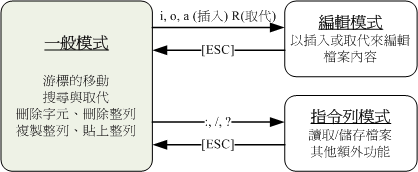
\includegraphics[scale=0.6]{pics/vi-mode} \\
最好用vim命令启动vi, 这个功能更强大一些。上面这个图非常重要,你需要经常点击i,如果进入插入模式,底部会出现--insert--的字样,
否则就是一般模式了。所有的编辑控制(拷贝粘贴等)命令都需要回到一般模式(通过esc来完成。)理解了三个模式, 就可以很好的使用vim了。
	\item common mode \\
	\begin{center}
		\begin{tabular}{c|c}
		\hline
		move & \\
		\hline ctrl+b & previous page\\
		ctrl+f & next page\\
		1G &  begin of document\\
		G & end of document\\
		0& begin of line \\
		\$ & end of line \\
		\hline
		copy & \\
		\hline v & begin to select\\
		y & copy\\
		d & delete\\
		p & paste \\
		yy & copy the whole line \\
		\hline
		delete & \\
		\hline x & delete one\\
		X & delete previous\\
		\hline
		search & \\
		\hline /word & find word\\
		?word & find word previous\\
		n & continue\\
		N & Continue previous\\
		\hline
		\end{tabular}
	\end{center}
	\item command mode \\
	\begin{center}
		\begin{tabular}{c|c}
		\hline :w & write \\
		\hline :q & exit \\
		\hline :! & force (!放到最后)\\
		\hline :n & next document \\
		\hline :N & previous document \\
		\hline :files & show how many files \\
		\hline :sp & 2 windows open files \\
		\hline ctrl+w (release) up arrow & upper window \\
		\hline ctrl+w (release) down arrow& down window \\
		\end{tabular}
	\end{center}

	\end{itemize}




\section{Version Control}
By now,  there is two famous websits, one is code.google.com, the other is github.com. They provides the version control function, and help to manage your source code and documents. the previous one support SVN, the latter one apply git. So, I will introduce these two systems together.
一个最根本的原则,如果单人开发,改动前,必须update, 如果多人开发,除了改动前必须update外,commit前也必须update, (这是因为这个阶段可能别人已经commit了一个新的版本)
\subsection{git}
\subsubsection{basic}
\begin{itemize}
\item 我在github有两个账号,zhaoyan.hrb@gmail.com zhaoyan;yan.zhao.74@gmail.com YanZhao. 有一个项目hello-world,主项目在zhaoyan上,然后我用YanZhao这个账号fork了一下。
zhaoyan上的项目超链接
git://github.com/zhaoyan/hello-world.git(只读版本) git@github.com:zhaoyan/hello-world.git

YanZhao上的项目超链接
git://github.com/YanZhao/hello-world.git(只读版本) git@github.com:YanZhao/hello-world.git


\item The two charactristics about git is \textbf{Distribute} and \textbf{Branch}, Distribute support working offline, Branch can make you manage branch easily and efficiently.
\item \textbf{所有的版本控制,都需要特别注意一个事情,不要取中文的文件名,如果你的英文非常不好,那就用拼音取文件名好了。 这点请务必要注意。}
\item In order to do anything in Git, you have to have a Git repository. This is where Git stores the data for the snapshots you are saving. There are two main ways to get a Git repository. \textbf{One way} is to simply initialize a new one from an existing directory, such as a new project or a project new to source control. \textbf{The second way} is to clone one from a public Git repository, as you would do if you wanted a copy or wanted to work with someone on a project.
\end{itemize}

\subsubsection{github.com}
\begin{itemize}
	\item build a account in github.com \\
		  YanZhao  yan.zhao.74@gmail.com   password for BBS
	\item \linuxcommand{ssh-keygen -t rsa -C yan.zhao.74@gmail.com} \\
        	your public key has been saved in /c/Users/zhao/.ssh/id\_rsa.pub(for windows) ~/.ssh/(for Linux). Then you should paste the public key to the account in github.com. once you finish it, you can use command ssh git@github.com to test it. (github网站上面有更详细的说明。)\\ 你可以把is\_rsa.pub和is\_rsa两个文件拷贝到别的计算机上。这样就不用再另外的计算机上用ssh-keygen命令了。
         	(ssh -v will give you verbose information. you must restart ubuntu after you move id\_rsa to ~/.ssh)。
         

	\item It's a social website, you need to find some friends here and exchange idea. 中国有那些类似的github网站,目前我还不是很清楚。

    \item 有的时候,你看不到项目的超连接地址,可以点击右上角的小眼睛(watchers),也会出现pull request.
    
    \item 完成以上步骤以后,还需要在本地对git进行简单的配置,这样别人才知道你的具体信息,才能和你联系啊。
    
    \begin{verbatim}
	git config --global user.name "zhaoyan"
	git config --global user.email zhaoyan.hrb@gmail.com
	\end{verbatim}
\end{itemize}

\subsubsection{configure}
    \begin{itemize}
    \item windows下,.gitconfig会保存在C:$\backslash$Documents and Settings$\backslash$Administrator下
    \item 运行 git config --global core.editor notepad (在windows下配置成notepad,当热,你也可以选择任何一个你更喜欢的编辑器)
    \item git config --list 可以列出所有的你的配置,你可以进行查看。
    \end{itemize}
    you also can change the ~/.gitconfig file and add below content, it will customize your own git.(color and log alias is more useful)

\begin{verbatim}
[alias]
co = checkout
ci = commit -a
st = status
br = branch
oneline = log --pretty=oneline --since='2 days ago'
onelog = log -p -1
[color]
status = auto
branch = auto
ui = auto
[merge]
tool = kdiff3
[mergetool "kdiff3"]
path = C:/Program Files/KDiff3/kdiff3.exe
keepBackup = false
trustExitCode = false	
\end{verbatim}
    利用KDiff3程序可以利用图形化的程序界面来更改源代码级别上的冲突情况。使用起来也相对简单。\\
编辑.gitignore文件
\begin{verbatim}
# 注释
*.a #忽略所有.a结尾的文件
!lib.a #但是lib.a除外
build/ #忽略build/下所有的文件
doc/*.txt #忽略所有doc/下的文本文件,但是doc/server/arch.txt会包括。
\end{verbatim}

在windows下,安装完成以后,运行git bash命令。可以配置成图形化的diff和merge。其中,下载P4Merge。基本的内容可以参考Pro Git第7章。其中,有一点需要注意,/D/Porgramm$\backslash$ Files/Perforce. 空格前面要加上反斜杠。当你运行git diff以后,就会弹出一个图形界面了。

\subsubsection{把一个已有项目加入到git}
        \begin{verbatim}
		cd test
		git init
		touch README
		git add README
		git add . 
//点代表所有的文件。Directories are added automatically when adding files inside them. That is, directories never have to be added to the repository, and are not tracked on their own. You can say "git add <dir>" and it will add files in there.
		git rm README1 (可以删除一个文件)
		git commit -m "first commit" ( you can't just give empty message)
		git commit -a -m "first commit"
		//这是一种比较简单的写法,综合了add 和commit 两个命令。但是,此处有一点应该注意,那就是git commit -a无法把新增文件或文件夹加入进来,所以,如果你新增了文件或文件夹,那么就要先git add newaddfile,再git commit。针对开发日志,第一行一定要是少于50字的开发概括信息, 而且第二行务必是空行,第三行开始才可以开始细致描述开发信息。 这是因为很多版本服务系统中的email机制都会选取log中的第一行为邮件题目。
		git log //提交完成以后,你可以用log命令检查一下,看看是否已经提交成功了。同时看看过去的历史,也挺有趣的!
        \end{verbatim}
        \textbf{然后,你必须先登陆到github,然后create repository, 名字叫做Other1}
        \begin{verbatim}
		git remote add origin git@github.com:YanZhao/Other1.git
		//origin 其实就是git@github.com:YanZhao/Other1.git的别名,
		git remote show
		//可以查看远端的repository情况。
		git push origin master 	
        //不能省略origin 和master 最好把这个命令写全。master 是默认本地存在的一个分支,你不用显式创建它。
		//这个命令把本地的内容“推”到服务器端。
		//you must have private key file for ssh in those case, you can copy it from ~/.ssh
		\end{verbatim}

\subsubsection{git基本图解}
 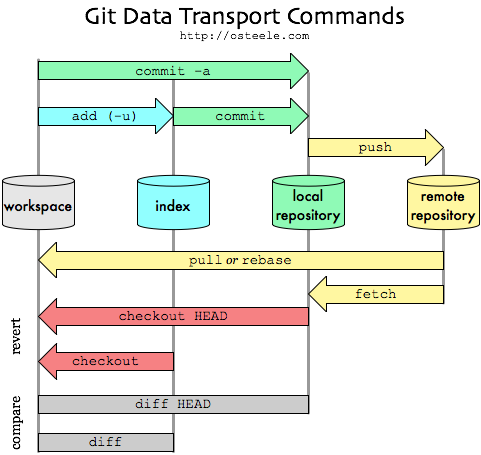
\includegraphics[scale=0.8]{pics/git-transport} \\

\subsubsection{基本命令}
\begin{itemize}
\item status 命令 \\
    这个命令应该算是所有git命令中最常用的一个命令了。应该随时随地的运行它。\par
    git status -s 会给出相对简短的命令,其中有两列,第一列位staging,第二列位working tree。如果你修改了a文件,然后add了,然后又修改了a文件。这个时候,运行git status -s
    会出现 MM a 的标志。具体什么含义,自己去想吧。

\item 提交命令add commit
    \begin{verbatim}
    将 Current working directory 记为 (1)
    将 Index file 记为 (2) 或者叫做 staging
    将 Git repository 记为 (3)

    git add .  //include all untracked file
    git reset -- a.c //从index file中删除掉登记的a.c
    git add -i  //interactive, you can select files to add, 
    select 4[add untraced] first  
    
    git add -u  //not add untracked file

    他们之间的提交层次关系是 (1) -> (2) -> (3)
    git add完成的是(1) -> (2)
    git commit完成的是(2) -> (3)
    git commit -a两者的直接结合

    时间上看,可以认为(1)是最新的代码,(2)比较旧,(3)更旧
    按时间排序就是 (1) <- (2) <- (3)

    此命令将使用当前的暂存区域快照提交。如果刚才提交完没有作任何改动,直接运行此命令的话,相当于有机会重新编辑提交说明,而所提交的文件快照和之前的一样。
启动文本编辑器后,会看到上次提交时的说明,编辑它确认没问题后保存退出,就会使用新的提交说明覆盖刚才失误的提交。
如果刚才提交时忘了暂存某些修改,可以先补上暂存操作,然后再运行 --amend 提交:

    git commit -m 'initial commit'
    git add forgotten_file
    git commit --amend
    \end{verbatim}

\item 文件改名和删除
\begin{verbatim}
rm a
git rm a
git commit -m "delete file a"

git mv a b 等同于mv a b  git rm a  git add b 三个命令
git commit -m "rename a to b"
\end{verbatim}
\item checkout命令
        \begin{verbatim}
git gc //每个月或者每100次commit就运行这个优化历史的程序。
git checkout  //如果没有给文件名,有点类似于(status)命令,只是告诉你一些基本的状态

git checkout . or git checkout file //(update from stage)
git checkout HEAD .  //( update from repo) .代表所有文件。

你可以从多个地方checkout 一个文件,这个有点意识。
git checkout v1.2.3 -- filename
# tag v1.2.3
git checkout stable -- filename
# stable branch
git checkout origin/master -- filename
# upstream master
git checkout HEAD -- filename
# the version from the most recent commit
git checkout HEAD^ -- filename
# the version before the most recent commit
如果你再(1)处更改了代码,你还可以分别从(2)和(3)处或者以上多个地方恢复回来旧的代码。不过你的更改的代码将会永久丢失,
所以以上这些命令要谨慎使用。如果你想保留你的更改。你可以首先:

git add filename 当前更改保存到index
git checkout v1.2.3 filename  得到以前的版本
git diff 比较不同
git checkout filename 再恢复到当前更改。

git checkout HEAD .
# 將所有檔案都 checkout 出來(最後一次 commit 的版本),
注意, 若有修改的檔案都會被還原到上一版. (git checkout -f 亦可)
git checkout xxxx .
# 將所有檔案都 checkout 出來(xxxx commit 的版本, xxxx 是 commit 的編號前四碼), 注意, 若有修改的檔案都會被還原到上一版.
git checkout -- *
# 恢復到上一次 Commit 的狀態(* 改成檔名, 就可以只恢復那個檔案)

\end{verbatim}

\item 比较命令 diff \\
 git fetch 更新以后,你可以利用git diff master origin/master查看一些有哪些改动了。来决定是否你要merge。所以说,fetch+merge比起pull来说更好一些,因为他能停留一下,给你检查一下的机会。 \par
 git diff 的输出中,a代表staging的文件,用-号标注,而b代表working tree的文件,用+号标注。
 \par
    \begin{verbatim}
git diff得到的是从(2)到(1)的变化
git diff –cached得到的是从(3)到(2)的变化
git diff HEAD得到的是从(3)到(1)的变化
git diff tag                    比较tag和HEAD之间的不同。
git diff tag file               比较一个文件在两者之间的不同。
git diff tag1..tag2             比较两个tag之间的不同。
git diff SHA11..SHA12           比较两个提交之间的不同。
git diff tag1 tag2 file or
git diff tag1:file tag2:file    比较一个文件在两个tag之间的不同。

tag可以remote的一个别称,
git remote add xjsff git://github.com/xjsff/hello-world.git
git diff xjsff/master README 查看当前README这个文件与xjsff/master中的README的主要区别。
    \end{verbatim}

\item 远端命令remote \\
\begin{verbatim}
git remote add paul git://github.com/paul/test.git
git remote -v
git remote show paul 显示paul的详细信息,包括分支
git remote rename paul pa
git remote rm pa 删掉pa,因为pa已经不再位项目做贡献了。
\end{verbatim}

\end{itemize}

\subsubsection{history 查看}
\begin{itemize}
\item revision \\
    \begin{verbatim}
    HEAD,FETCH_HEAD,ORIG_HEAD, MERGE_HEAD, COMMIT_EDITMSG:最后一次commit时的提交信息。
    HEAD:表示最近一次的commit。
    MERGE_HEAD:如果是merge产生的commit,那么它表示除HEAD之外的另一个父母分支。
    FETCH_HEAD:使用git-fetch获得的object和ref的信息都存储在这里,这些信息是为日后git-merge准备的。
    HEAD^:表示HEAD父母的信息 等于ORIG_HEAD

    ^ commit对象的第一个父母
    HEAD^^:表示HEAD父母的父母的信息
    HEAD^1:表示HEAD的第一个父母的信息
    HEAD^2:表示HEAD的第二个父母的信息

    ~n commit对象的上溯n代的父母
    HEAD~4:表示HEAD上溯四代的信息,~加数字。

    HEAD:README.txt 代表一个blob对象了。(blob对象的sh-hash值一般看不到,也不方便引用)

    :/fix a bug #代表在commit message 中查找fix a bug有这个串的第一个commit

    @{date specification}
    HEAD@{yesterday}

    git log 后面跟随一个命令集,命名一个集合可以采用一些简写。
    1)B...C #the set of commits that are reachable from either one of r1 or r2 but not from both.
    2)^G D #D的所有父母(包括D),但是不包括G的这个分支。
    3)D F #D,F的所有父母(包括D,F)
    4)C^@ #C的所有父母(不包括C)
    5)
    详细的信息,可以进一步参考gitrevisions命令
    \end{verbatim}

\item blame
    \begin{verbatim}
    git blame -L l2,l3 hello.html
    \\会给出那些行是由那些行提交的。这个信息非常的具体。可以帮你找到元凶to blame。
    \end{verbatim}

\item log
    \begin{verbatim}
    git的历史记录是由一些列相关联的”commit”所组成的。每一次“commit”都会有一个唯一的名称(hash值) 我们可以使用git show再加上hash值显示具体的某次提交。你完全可以用一个最短的且唯一的“名称前几个字符”来只待某次commit:

    git log:显示commit日志
    git log -p:不仅显示commit日志,而且同时显示每次commit的代码改变。
    git log -p -2: 这个命令比较常用,他只显示最近的两次更新。
    git log --oneline 显示简略信息。
    git log --abbrev-commit --pretty=oneline #显示简略的信息
    git log experiment..master #表示的是在master上而不在experiment上的提交。
            a--b--e--f(master)
                \c--d(experiment)
    git log origin/master..HEAD #你将把什么推送到远程。
    git log --left-right master...experiment 显示每个提交属于那一侧的分支。三点代表所有master和experiment分支中的提交。
    \end{verbatim}
\item stash
    \begin{verbatim}
    你正在工作,还么有完成,这个时候,老板让你紧急修改一个release版本的bug,这个时候,stash,然后checkout release. 工作完毕,commit,这个时候git stash pop.

    git stash save “you messaage" #这样可以引入相应的提示信息。
    git stash list #列出所有的stash。
    git statsh pop #如果发生冲突,会自动merge失败。这个时候,需要你手工解决冲突。

    \end{verbatim}
\item show
    \begin{verbatim}
    使用git show加分支名称,亦可以显示分支信息:
    git show master
    git show experimental

    使用HEAD字段可以代表当前分支的头(也就是最近一次commit):
    git show HEAD:README.txt #显示某次提交的README.txt的文件内容。这个时候你不用checkout出来了。
    当然,你也可以重定向到某个文件。例如 git show HEAD:README.txt >OLDREADME.txt文件。
    git show HEAD #同时显示当前提交和上一次提交的差异。
    git show 23df7 (版本号的前五位)
    每一次commit都会有”parent commit”,可以使用^表示parent:
    git show HEAD^ //查看HEAD的父母的信息
    git show HEAD^^ //查看HEAD的父母的父母的信息
    git show HEAD~4 //查看HEAD上溯4代的信息
    要注意的是git-merge是会产生双父母的,这种情况这样处理:
    git show HEAD^1 //查看HEAD的第一个父母
    git show HEAD^2 //查看HEAD的第二个父母


    你可以给复杂名称起个别名:
    git tag V3 5b888 //以后可以用V3来代替复杂的名称(5b888…)
    git show V3
    git branch stable V3 //建立一个基于V3的分支

    可以用git grep帮助我们搜索:
    git grep “print” V3 //在V3中搜索所有的包含print的行
    git grep “print” //在所有的历史记录中搜索包含print的行
    \end{verbatim}
\end{itemize}

\subsubsection{图形界面}
    \begin{itemize}
    \item gitk是一个图形界面程序,你可以查看具体的分支情况。也可以进行一些命令行才能完成的工作。
    \item gitk --all 会列出所有的分支。如果没有--all好像只列出当前的分支。
    you need to understand the basic the meaning of the basic command, so there is a figure below to illustrate it. \\
    \item KDiff3是一个图形化的文件合并工具。使用前需要在.gitconfig文件中进行相关的设置。
    \end{itemize}

\subsubsection{history恢复}
\includegraphics[scale=0.6]{pics/git-history} \\

恢复历史版本: \\
\begin{verbatim}
git commit -C HEAD -a --amend,对最后一次提交做一些修改。(只对最后一次修改有效)
git revert HEAD^^ 会产生一个新的commit。

0)add a,但是发现不想把a置于git控制中,可以用git reset -- a. 
如果已经提交了,可以git rm a. 他会从index file中删除,但是working diretory 中保留a
然后重新提交就可以了。

1)刚刚修改还没有提交
git reset HEAD a.c add了,但没有commit. 取消掉add的内容
git checkout -- a.c  修改了,但是没add,取消掉修改的内容。

2)把某个文件恢复到过去
git checkout HEAD^^ a.c

3)暂时回到过去
git checkout HEAD^^
git chekcout -b dirty
你可以实验,修改等然后
git checkout master

4)永远回到过去
git rest --hard HEAD^^

5)把branch1的历史完全写入到当前的分支当中去。
git rebase branch1
\end{verbatim}



\subsubsection{tag 打标签}
\begin{verbatim}
tag的名字不能包含空格。
建立release branch: git branch RB_1.0
进行一些打包和测试,然后打上标签 git tag 1.0
删掉git branch -D RB_1.0
如果还需要修改这个release, 就
git branch RB_1.01 1.0
git checkout RB_1.01
修改 commit.
git tag 1.01 继续打一个新标签。
git branch -d RB_1.01 删掉这个新的分支。

git archive --format=tar \
--prefix=mysite_release/ \
HEAD | gzip >mysite_relase.tar.gz
//把最后的产品进行打包。
\end{verbatim}


\subsubsection{branch}
分支的的基本命令
\begin{verbatim}
git branch -r 会列出所有remote tracking分支
git branch //会列出当前全部的分支,所在分支会用星号来表示。\\
git branch -D b1 //会删除掉b1这个分支。\\
git checkout branch-name // 切換到 branch-name\\
git checkout -b new-branch master // 從 master 建立新的 new-branch, 並同時切換過去 new-branch\\
git checkout -b newbranch / 由現在的環境為基礎, 建立新的 branch\\
git checkout -b newbranch origin // 於 origin 的基礎, 建立新的 branch\\
git branch -m master mymaster //重命名master为mymaster.(没什么意义) \\
git push origin branch ,//this command will push branch to github. \\
but push branch to server isn't very meaningful, at least I think so. \\
\end{verbatim}

分支的基本知识:\par
1) 主要有两种分支,一种是本地分支,你可以用git branch来查看他们;另外一个就是remote-tracking branches,你可以用git branch -r来查看他们。他们一般的样子类似于:origin/albert和origin/master。你需要注意,origin是源的别名,而不是分支的名字,albert才是真正的分支的名字。\par

2)git push origin experiment \#把一个分支推送到服务器:\\
git push origin local:experiment \#把本地分支改名,推送到服务器端,服务器端分支名为experiment. \\
git push origin :experiment \#把一个分支删除掉,(用空名改名) git push origin erperimental:experimental-by-yan 给remote-tracking-branches另外的名字,这里experimental-by-yan是remote-tracking-branches名字,erperimental是本地分支的名字。 这种方式叫做<source-name>:<destination-name> \par

3)对于remote-tracking branches,你不能直接在上面操作,你可以用git fetch 来 update。或者是与你当前branch merge。或者基于他创建本地分支。\\
git chekcout -b refactored origin/refactored \par
git checkout --track -b refactored origin/refactored (注意有--track).以上两个命令应该大致作用一致。 \par



分支的基本原则:\\
one branch is for (master), one is for merge, the others is for daily experiments. when you want to emerge other's work, you need to build a branch.\\

分支是根据当前的commit 的内容来建立的,而不是根据working tree 或者是index。所以你在merge前,最好先要commit才行。\\

一个分支和主分支merge以后,最后就把它删掉,然后从主分支在创造出一个分支。这样管理起来比较舒服,不要给自己找麻烦。\\

\subsubsection{merge}
分支的合并:\\
\begin{itemize}
\item git merge-base b1 b2 发现b1和b2的共同祖先
\item git cherry -v master test 在master分支中,找到所有test中有但是master中没有的commit.
\item git-merge主要用于将两个或两个以上的开发分支进行合并。主要有三种merge.第一种为straight merge. 他把一个分支的整个历史合并到另外一个分支当中去。还有一种就是squash 把所有的历史变成一个历史commit。 git merge --squash contact。针对于squash,你需要merge以后再提交。最后一种就是cherry-pick,git chekcout master git cherry-pick 321d76f (这是在另外一个分支提交的)。 当然1你也可以git cherry-pick -n 321d76f. -n 告诉git先不提交,然后你就可以继续cherry-pick了。 然后 git commit 不用-m,这个时候一个默认的编辑器就打开了。所有你pick的commit message就会自动出现在那个编辑器中。

\item git merge branchname 用于将branchname分支合并到当前分支中。如果没有冲突,就把分支的commit forward到当前分支中,也就是相当于产生了新的commit。 如果合并发生冲突,需要自己解决冲突)

\item 当merge命令自身无法解决冲突的时候,它会将工作树置于一种特殊的状态,并且给用户提供冲突信息,以期用户可以自己解决这些问题。当然在这个时候,未发生冲突的代码已经被git merge登记在了index file里了。如果你这个时候使用git diff,显示出来的只是发生冲突的代码信息。

在你解决了冲突之前,发生冲突的文件会一直在index file中被标记出来。这个时候,如果你使用git commit提交的话,git会提示:filename.txt needs merge
在发生冲突的时候,如果你使用git status命令,那么会显示出发生冲突的具体信息。\\
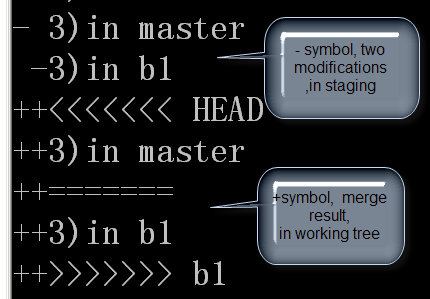
\includegraphics[scale=0.6]{pics/merge-diff} \\

在你解决了冲突之后,你可以使用如下步骤来提交:
第一步:git add filename.txt
第二步:git commit

\item 如果你希望撤销一个分支到merge前的状态,那么使用如下命令:\\
git reset –hard HEAD \\–hard表示将working tree和index file都撤销到以前状态。
Or, if you've already committed the merge that you want to throw away, use this command: git reset --hard ORIG\_HEAD \\
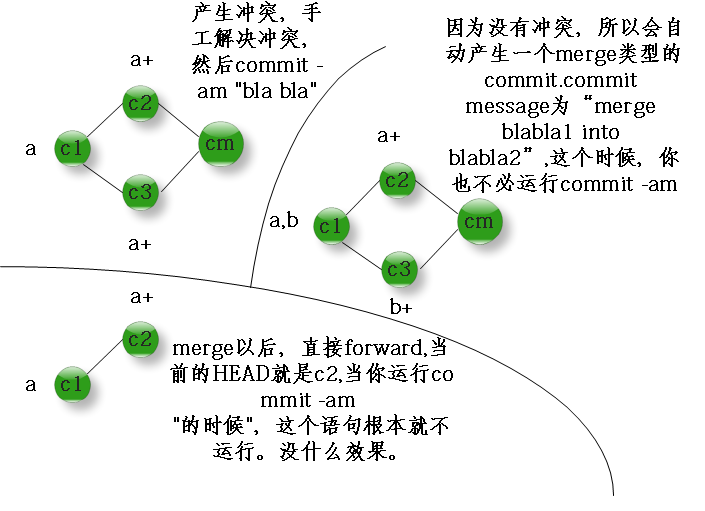
\includegraphics[scale=0.5]{pics/git-merge} \\
\end{itemize}

\subsubsection{reset}
git reset –hard HEAD //–hard表示将working tree和index file都撤销到以前状态。–soft表示只撤销commit,而保留working tree和index file的信息,–mixed会撤销commit和index file,只保留working tree的信息。 这里-mixed是reset的默认选项。

回退掉刚才提交的一个commit. 利用
\begin{verbatim}
git reset -soft HEAD^
\end{verbatim}
git diff返回空,而git diff –cached和git diff HEAD会返回有效信息。这说明使用–soft选项后,只回退了commit的信息,而不会回复到index file一级。哈哈,这就说明了你如果想撤销commit,并且只回退commit的信息,那么就用 -soft吧!

\subsubsection{rebase}
\textbf{Never rebase branches or trees that you pulled. Only rebase local branches. Never ever rebase a branch that you pushed, or that you pulled from another person} \par
rebase的命令和merge的命令有点不太一样。一个标准的流程应该是从master创造出一个分支test,然后在test commit 几次。同时在master commit 几次。这个时候,进入master分支,git rebase test, 或者进入master以后,用merge test, 把test的工作集成到master中去。然后删除test分支。这个就是git的主要工作流程。从这里,你也可以看到 rebase 和merge之间的不同。merge会丢到所有在test分支中的历史。而rebase把这个分支中的历史写道master中了。
 因为他会改变hash的值。可以参考我的网络书签的说明。我一般个人开发,产生一个branch后,master就不变了。 这个时候使用merge 和rebase都是可以的,关键就是你是否对test中的commit的那些历史感兴趣。还有一种流程就是通常 git rebase 1.0

rebase的具体工作流程可以参看这个例子:git rebase test \\
1. 先将test 分支的代码checkout出来,作为工作目录 \\
2. 然后将master分支从test分支创建起的所有改变的补丁,依次打上。如果打补丁的过程没问题,rebase就搞定了 \\
3. 如果打补丁的时候出现了问题,就会提示你处理冲突。处理好了,可以运行git rebase –continue继续直到完成 \\
4. 如果你不想处理,你还是有两个选择,一个是放弃rebase过程(运行git rebase –abort),另一个是直接用test分支的取代当前分支的(git rebase –skip)。 \\

\includegraphics[scale=0.7]{pics/git_rebase} \\

1)如果b是一个本地的branch,如果master上没有m1那么在master 上,执行 git rebase b 和git merge b效果一样,就是增加两个新的commit。 \\

2)如果master 上也有个更新m1。那么需要注意,如果m1只是本地的(你不是pull,同时,你还没有push)同时,你还希望保存
b1 和 b2 两次commit。这个时候,可以使用git rebase b. (因为m1 hash值改变了,所以必须要保证本地化)。\\
3)如果master上m1不是本地化的,那么你最好用merge。但是当你删掉b分支以后,b1,b2消失了。\\

4)如果master上m1不是本地化的,你也可以进入b分支, 然后git rebase master,(不过你需要注意,这个时候,你还在b分支里面。)然后git checkout master , git merge b。
相当于把b当中的b1和b2,放到了m1前面,(m1的hash没变,相当于增加了两个新的commit b1和b2. 你还需要保证b是个本地的branch)
一句话:rebase的使用需要谨慎使用,他的本意是修改历史的作用,如果你没有很明显的理由,就直接用merge好了。\\

rebase branch1 有三个含义,1)当前不再branch1中,2)branch1为焊接接入点,3)当前的分支commit的值改变了。

rebase branch 与rebase master是有区别的。如果你当前在master中,并且以master为主线,那么就应该调用rebase branch。从这个角度上来说,rebase master应该用的不多。除非是上面说的第4种情况,那就是m1已经push出去,并且别人也在用。

rebase两种常用场景,第一就是本地的分支上,两个分支出现并行情况,通过rebase branch1,可以得到相对干净的历史commit. 第二就是rebase thorn/master, 把别人的工作集成到我的master中去,(thorn/master和master都发生了commit)生成一个更干净的历史。他的基本原理和merge大致相同。

\subsubsection{与人合作}
singel person, center control, with branch \\
	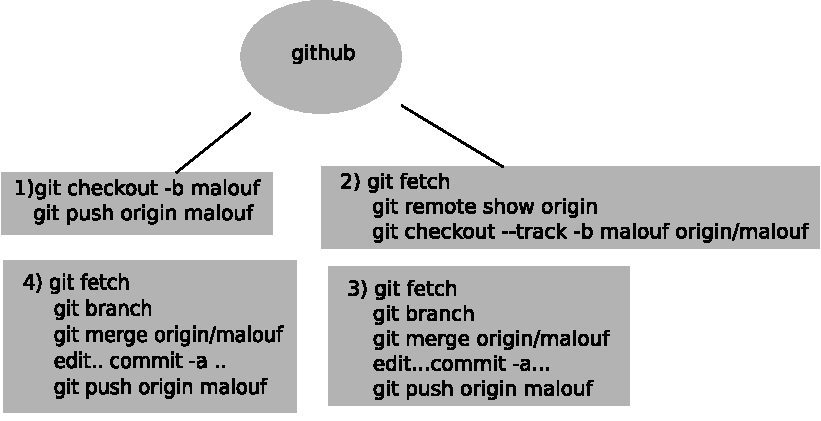
\includegraphics[scale=0.6]{pics/git_branch} \\
   	when you finish the branch, you can merge it with master.

\subsubsection{基于分支合作开发}
\begin{verbatim}
1)git fetch upstream #得到zhaoyan的主线最新开发进展。

2)git checkout -b test_bla upstream/master #以zhaoyan的主线最新开发分支master进展为基础,建立本地的topic分支test_bla (自己想个合适的分支名字,带有描述性。)

3)edit... compile....
   git commit -am "s1"
   edit... compile....
   git commit -am "s2" #你的工作过程可能花费几天,或者几个小时。在这个过程中,upstream/master也许发生了变化,zhaoyan也许在upstream/master提交了新的更新t1。这个时候,commit有以下的历史:

     s1--- s2
____/___t1

4)git fetch upstream #完成你的开发任务以后,你想把你的工作贡献给zhaoyan,这个时候,你需要再次得到zhaoyan的主线最新开发进展。(因为你提交s1和s2的时候,zhaoyan同时在upstream/master上提交了t1)如图。

5a)得到最新的进展以后,你可以使用两种方法,第一种就是利用merge方法。
git merge upstream/master
	如果没有冲突,forward或者自动生成一个merge commit.
	如果有冲突,手工解决你的冲突以后,git commit -am "st1"

     s1--- s2
____/___t1___\st1______


5b)得到最新的进展以后,你可以使用两种方法,第二种就是利用rebase方法。
git rebase upstream/master
	如果没有冲突,forward 或者自动生成一个commit.
	如果有冲突,手工解决你的冲突以后,git add conflict_file 然后git rebase --continue,(不用调用git commit了)。commit历史如下图所示。如果同学们不理解rebase命令的具体含义,请优先选择merge命令。rebase命令具有一定的风险性。

     t1---s1--- s2
____/


6)git push origin test_bla

7)登录到github网站上,找到hello-world项目,切换到test_bla分支。去找那个该死的request pull按钮并点击它。

8)如果zhaoyan已经处理了你的request-pull,并且把你的test_bla集成到zhaoyan的工作中,那么日后,你就可以删掉test_bla这个分支了。git branch -D test_bla

9)git push origin  :test_bla删掉github上的test_bla分支。

10)至此,一个开发流程结束,如果你想开始一个新的开发流程,可以从第1)到9)步重新开始,获得最新进展,重新建立一个新的分支, 完成以后,给zhaoyan发request-pull等等。
\end{verbatim}

\subsubsection{VS2010}


\subsubsection{codeblock}
0)项目文件为pro1.cbp文件,同时,所有源文件也保存到这里,当你编译的时候,会生成两个文件夹
第一个文件夹为bin,第二个文件夹为obj,你可以定义或修改.gitignore文件,加入 bin/ 和obj/。这样在提交的时候就会忽略掉这两个目录。相对来说比较简单。

\subsubsection{kdevelop}
你可以参考如何利用svn,这里重要的不是了解git,而是要理解kdevelop是如何管理一个项目的。\\
0) rm Makefile.in or .svn (if there are) \\
1) go into the src directory, and run git init \\
2) git add * \&\& git commit \\
3) git remote add origin git@github \\
4) git push origin master \\

0) another kdevelop, rm src\\
1) git clone git@github src\\
2) modify Makefile.am with you kdevelop project file.\\
3) in configure dialog, Configure options->linker flager -> add -L./ and add lib to the debug/src directory.\\
4) compile and run.\\

\subsubsection{single person on different computers }
\begin{itemize}
	\item Computer1...
    \begin{verbatim}
    git log HEAD..origin \\查看是否有区别,如果有就fetch,merge。
    git fetch
    git merge origin
    ( git fetch give you more chance to examing it, it's better)
    git commit -a -m " "
    git push
    git log HEAD..origin \\检查是否push成功。
    \end{verbatim}
    \item Computer2...
    \begin{verbatim}
    同样的操作,这里merge的时候,只会产生forword merge,情况相对比较简单。
    \end{verbatim}
\end{itemize}

\subsubsection{cooperation}
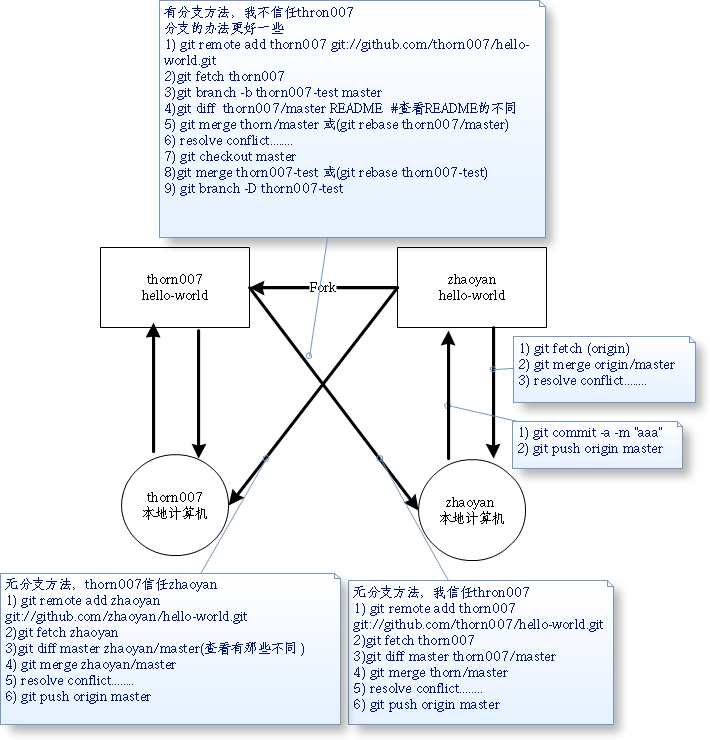
\includegraphics[scale=0.8]{pics/git-corp} \\
\begin{verbatim}
基本命令如下:
git fetch /home/bob/myrepo master:bobworks //用于从bob的工作目录的master分支下载到本地的bobworks分支中。
git-pull的作用就是从一个repository取出内容并合并到另一个repository中。
git pull是git fetch和git merge命令的一个组合。
git pull /home/bob/myrepo 这个命令的意思是从此目录中取出内容并合并到当前分支中。
git pull .就相当于git merge。

下面我给出一个具体的例子:
当合作伙伴bob希望改进我(rocrocket)的工作成果,则:
$git clone /home/rocrocket/project myrepo //此命令用于克隆我的工作到bob的myrepo目录下。请注意,此命令有可能会因为/home/rocrocket的目录权限问题而被拒绝,解决方法是chmod o+rx /home/rocrocket。
(省略bob数小时的开发过程)…
$git commit -a //bob提交自己的改进成果到自己的git仓库中,并口头告知我(rocrocket)他已经完成了工作。

我如果非常信任bob的开发能力:
$ cd /home/rocrocket/project
$ git pull /home/bob/myrepo //pull命令的意思是从远端git仓库中取出(git-fetch)修改的代码,然后合并(git-merge)到我(rocrocket)的项目中去。读者要记住一个小技巧,那就是“git pull .”命令,它和git merge的功能是一样的,以后完全可以用git pull .来代替git merge。请注意,git-pull命令有可能会因为/home/bob的目录权限问题而被拒绝,解决方法是chmod o+rx /home/bob。


如果我不是很信任bob的开发能力:
$ cd /home/rocrocket/project
$ git fetch /home/bob/myrepo master:bobworks //此命令意思是提取出bob修改的代码内容,然后放到我(rocrocket)工作目录下的bobworks分支中。之所以要放到分支中,而不是 master中,就是要我先仔仔细细看看bob的开发成果,如果我觉得满意,我再merge到master中,如果不满意,我完全可以直接git branch -D掉。
$git whatchanged -p master..bobworks //用来查看bob都做了什么
$git checkout master //切换到master分区
$git merge bobworks
$git branch -D bobworks //如果我检查了bob的工作后很不满意,就可以用-D来放弃这个分支就可以了
过了几天,bob如果想继续帮助我开发,他需要先同步一下我这几天的工作成果,只要在其当初clone的myrepo目录下执行git pull即可:
#git pull //不用加任何参数,因为当初clone的时候,git已经记住了我(rocrocket)的工作目录,它会直接找到我的目录来取。
\end{verbatim}

	if modification is small , you can use email+patch; If the modification is big, you can use fork pattern
	\begin{itemize}
    \item you can clone a exist project from other's people or on other computers,
		\begin{verbatim}
		git clone git://github.com/YanZhao/YanZhaoDoc.git
        (this is for visitor clone);
		git clone git@github.com:YanZhao/YanZhaoDoc.git
        (this is for admin clone);
		\end{verbatim}
	\item email topic()
		\begin{verbatim}
		1) git clone http://www.bitsun.com/git/gittutorcn.git
		2) edit and commit
		//method 1 (develop on master)
		$ git  fetch origin
		$ git rebase origin
		$ git for1mat path origin  ->0001-your-buddy-s-contribution.txt
		//method 2 (develop on branche, better)
		$ git checkout -b patch_mubs
		$ git checkout master
		$ git pull
		…
		$ git checkout patch_mubs
		$ git rebase master ( why I need rebase here, I want to know answer)
		
		3)email 0001-your-buddy-s-contribution.txt to vortune@gmail.com
		for vortune:
		1) git checkout -b buddy-in
		2) git am /path/to/0001-your-buddy-s-contribution.txt
		\end{verbatim}
	\end{itemize}

    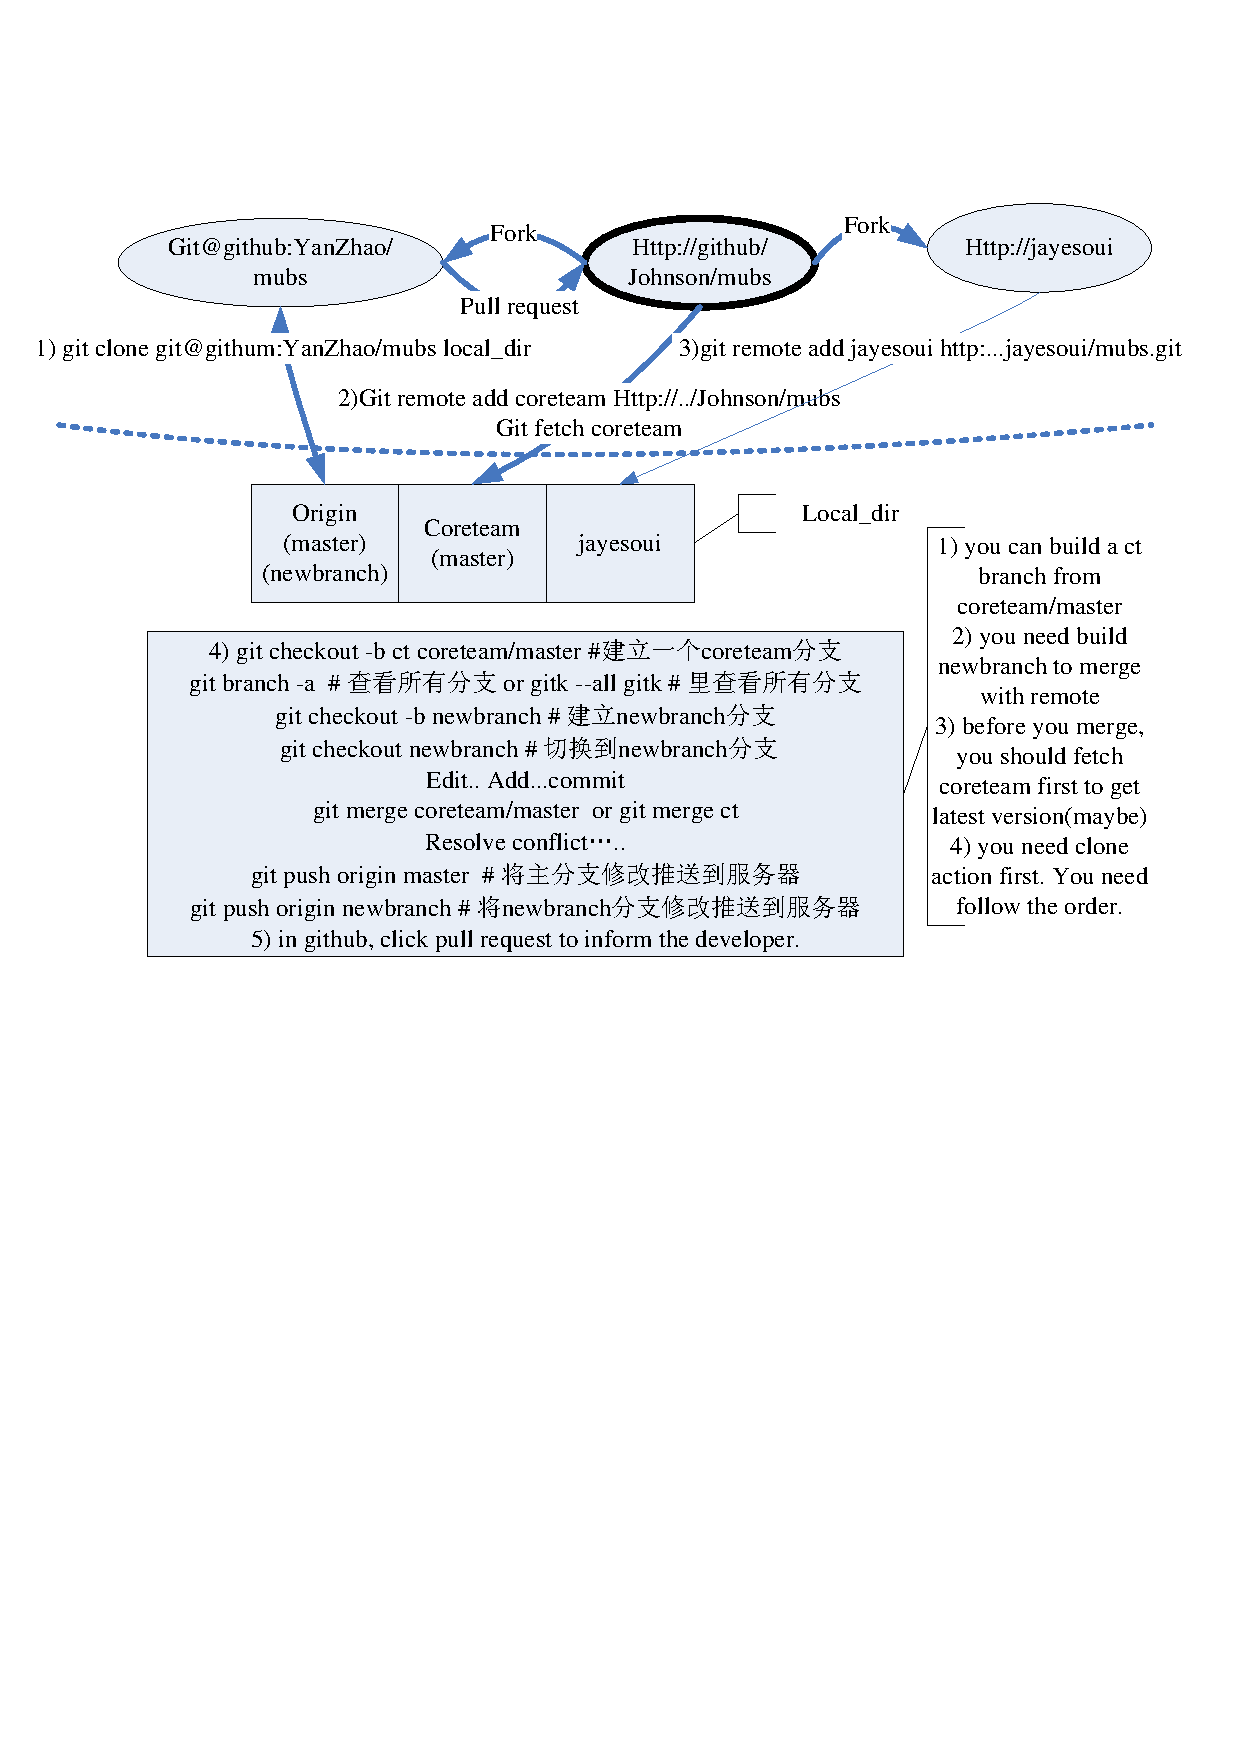
\includegraphics[scale=0.7]{pics/Visio-git_cooperate}

\subsection{SVN}
\subsubsection{basic knowledge}
	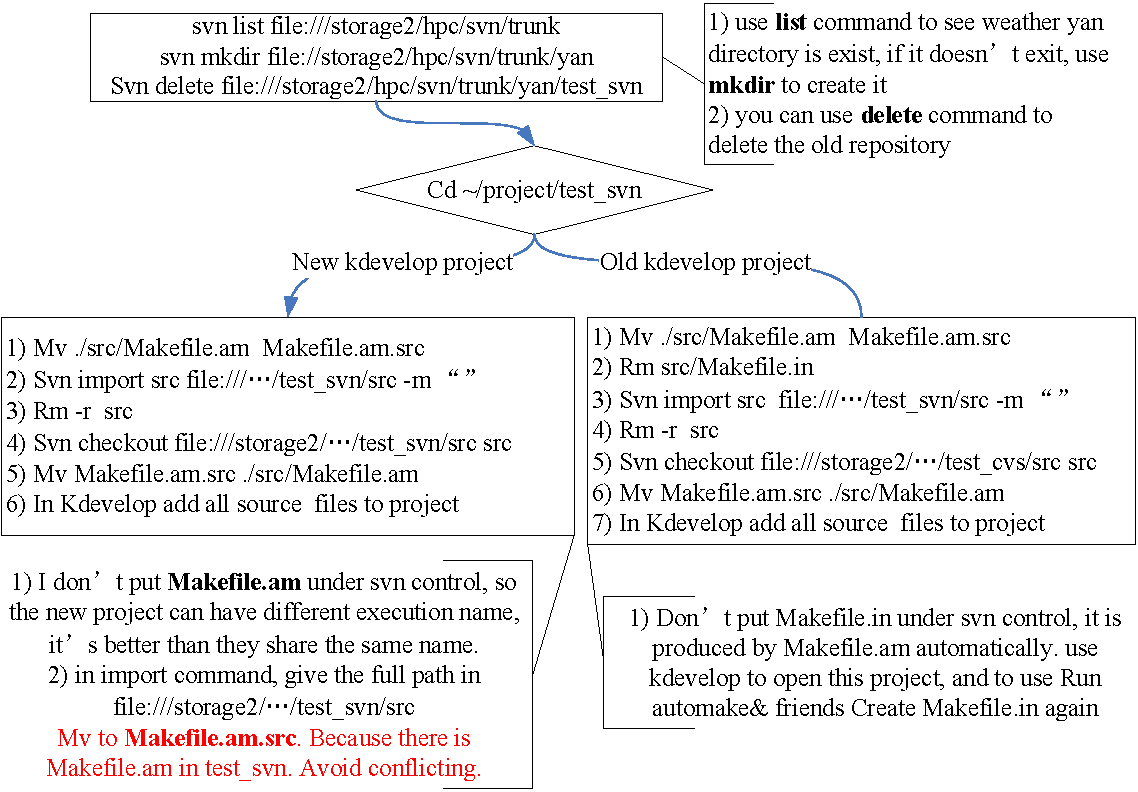
\includegraphics[scale=0.8]{pics/svn1_clip} \\
	 在svn下项目中,我并没有把Makefile.am放到版本控制下,其实,可以把它放到版本控制下, 只不过在新项目中引入的时候,你需要修改Makefile.am中的项目名字,使得他和你的新项目的名字一致就可以了。 \\

	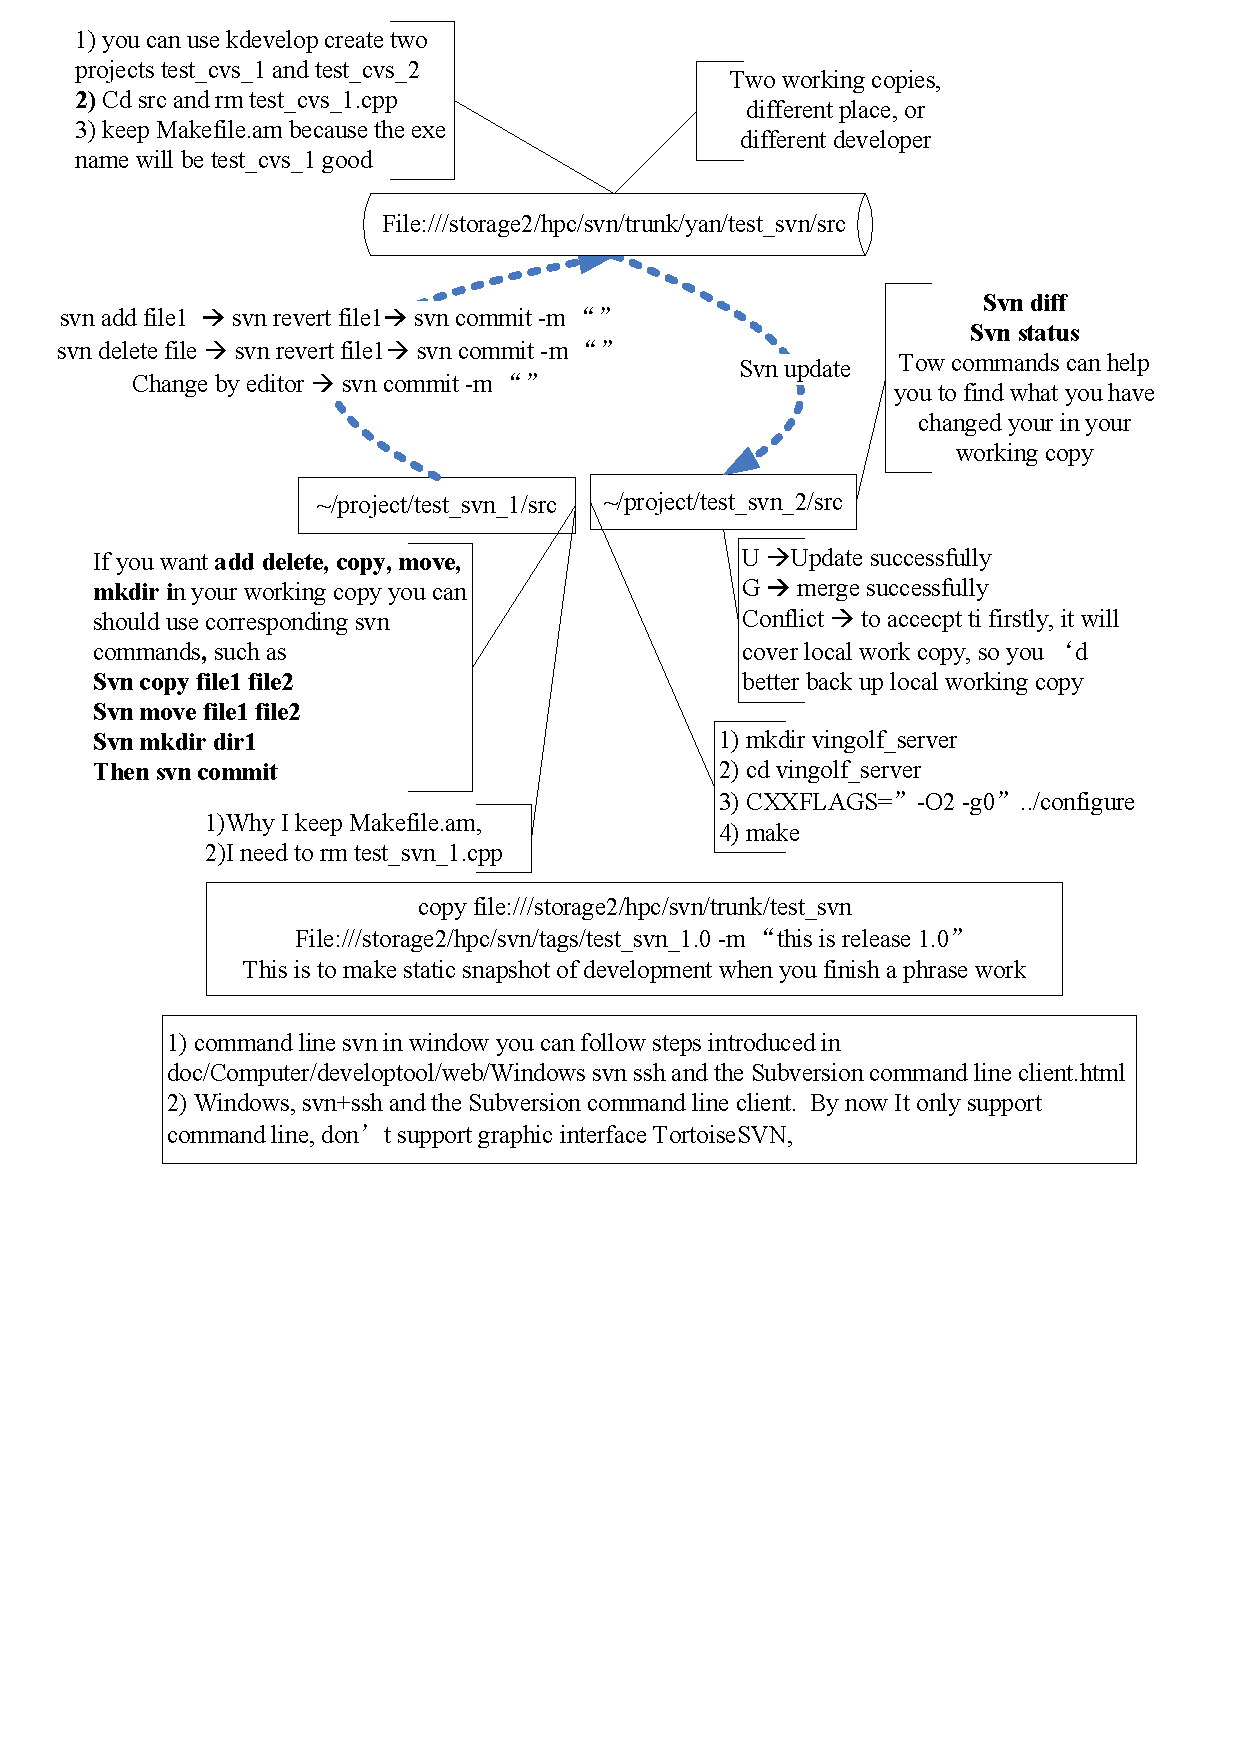
\includegraphics[scale=0.8]{pics/svn2_clip} \\

\subsubsection{common commands}
\begin{enumerate}
 \item update your working copy: \\
   svn update
 \item make changes: \\
    svn add \\
    svn delete dir \\
    svn copy \\
    svn move \\
    svn mkdir dir \\
    svn move src det \\
    svn list :to see which file has been added \\

\item Examing you change: \\
    svn status \\
    svn diff \\
\item undo:
    svn revert \\
\item reslove conflicts: \\
    svn update \\
    svn resolve \\
\item commit: \\
    svn commit \\
\end{enumerate}

\verb=/usr/bin/svn= is the most power tool , you need use it first.

\subsubsection{code.google.com}
\begin{itemize}
    \item svn import  a.file  https://yan-zhao-doc.googlecode.com/svn/trunk/a.file  -m " "
       (you must give the file name in the end of trunk, or it will not work)  \\
	svn import  dir  https://yan-zhao-doc.googlecode.com/svn/trunk/my\_dir  -m " "
	(you can change the dir name  in the end of trunk)
    \item for change: svn checkout https://yan-zhao-doc.googlecode.com/svn/trunk/ yan-zhao-doc --username yan.zhao.74 \\
for other: svn checkout http://yan-zhao-doc.googlecode.com/svn/trunk/ yan-zhao-doc-read-only
    \item  put your mature product in download tab.
\end{itemize}


\subsubsection{merge}
\begin{enumerate}
 \item copy: \\
svn copy http://svn/trunk/   http://svn/branches/new\_feature
\item chekcout:\\
svn checkout
http://svn/branches/new\_feature \\
wokr on new\_feature project with kdevelop
\item merge from trunk:\\
svn merge http://svn/trunk (if trunk is keep running) \\
 (resolve conflict, test, build) \\
svn commit
\item merge from branch:\\
go to trunk workcopy \\
svn merge  --reintegrate http://svn/branches/new\_feature \\
svn commit
\item delte the new feature branch:\\
cd new\_feature \\
svn delete \\
svn commit \\
rm new\_feature
\end{enumerate}

\begin{verbatim}
single merge
0) f:\\temp\\temp (r11)
1) F:\\>svn copy https://yan-zhao-doc.googlecode.com/svn/trunk/
https://yan-zhao-doc.googlecode.com/svn/branches/new\_feature -m "build a new feature\_branch"
( you must use https, not http) (r13)

2) F:\\temp\\>svn co https://yan-zhao-doc.googlecode.com/svn/branches/new\_feature
(it will build new\_feature directory)

3) cd f:\\temp\\new\_feature ->edit-> svn commit ...(r14 ,r15)

svn merge https://yan-zhao-doc.googlecode.com/svn/trunk/
(if trunk is still running)

4) cd f:\\temp\\trunk\\trunk svn merge --reintegrate
https://yan-zhao-doc.googlecode.com/svn/branches/new\_feature

5) svn commit (r16)

6) cd f:\\temp\\new\_feature -> svn delete
https://yan-zhao-doc.googlecode.com/svn/branches/new\_feature (r17)

7) rm f:\\temp\\new\_feature (delete local)
\end{verbatim}
用svn来建立分支和管理分支不是一个好主意,应该使用git。

\subsubsection{How to work under window}
By now commandline client 1.5.5 can work at my vista computer.
run cmd
and run svn co svn+ssh://yzhao@skuld/storage2/hpc/svn/trunk/yan/latex\_doc

\subsubsection{How Working Copies Track the Repository}
For each file in a working directory, Subversion records two essential pieces of information in the .svn/ administrative area:
      what revision your working file is based on (this is called the file's working revision), and
      a timestamp recording when the local copy was last updated by the repository.

Given this information, by talking to the repository, Subversion can tell which of the following four states a working file is in:
\begin{description}
\item[Unchanged, and current]
The file is unchanged in the working directory, and no changes to that file have been committed to the repository since its working revision. An svn commit of the file will do nothing, and an svn update of the file will do nothing.
\item[Locally changed, and current]
The file has been changed in the working directory, and no changes to that file have been committed to the repository since its base revision. There are local changes that have not been committed to the repository, thus an svn commit of the file will succeed in publishing your changes, and an svn update of the file will do nothing.
\item[Unchanged, and out-of-date]
The file has not been changed in the working directory, but it has been changed in the repository. The file should eventually be updated, to make it current with the public revision. An svn commit of the file will do nothing, and an svn update of the file will fold the latest changes into your working copy.
\item[Locally changed, and out-of-date]
The file has been changed both in the working directory, and in the repository. An svn commit of the file will fail with an ``out-of-date'' error. The file should be updated first; an svn update command will attempt to merge the public changes with the local changes. If Subversion can't complete the merge in a plausible way automatically, it leaves it to the user to resolve the conflict.	
\end{description}


\section{sed and awk}
sed is capable of editing task for file, awk is good at some format file and prodcue formate report.
they both can deal with a big file, while with interactive editor may need long time.
\subsection{sed}
	\subsubsection{General Knowledge}
		\begin{itemize}
		\item Firstly, I need to introduce the ed command, It's good start for a lot of useful text tool in linux.
		For example: \linuxcommand{ed test} will open the test file and go to the last line; default, the ed command will only
		be applied to the present line, but both sed and awk will loop all lines in a file. That is the most imporant difference
		in fact, grep means g/re/p command in ed, g means we deal with all lines, and p means print
		\item If there is syntaic error, sed will output command garbled.
		\item both sed awk give default loop for main input of file. It can help you to save some troubles. And they
		also support regular expression. That is two important characteristics when you use these two commands. awk has  two main
		differences with sed. The first one is it provide statements and you can controlthe processing by loop or judge (if..then).
		the second one it support field in a record. Means a word in a line by $1,$2. Sed work on the string level, tr work on the character level. Sed use argument, but tr use <filename.
		And sed can't work on ascII code.
		\item There is three basic displines of sed
			\begin{itemize}
			\item all commands are applied to each line
			\item a command is applied to all lines unless if you use address
			\item you didn't change origanl file, you need redirect to save changed result
			\linuxcommand{sed 's/aa/bb/' oldfile >newfile} then you can use \linuxcommand{diff -y oldfile newfile} to
			check the result.
			\end{itemize}
		\end{itemize}
	\subsubsection{Command Syntax}
	\linuxcommand{sed [options] 'script' file}
		\begin{description}
			\item[Options]: \\
			\begin{tabular}{c|p{0.5\textwidth}}
			\hline
			\op{n} & default, sed will output all lines. n means don't output any thing to the stdout unless you use p command
			For example \linuxcommand{sed -n ``s/old/new/p'' filename} only output those changed lines. \\
			\op{e} & means it followed by a script. When you input more scripts, you need it. \\
			\op{f} & specify the script file\\
			\hline
			\end{tabular}
		\item[Script]
			script is compsed of [address]command, I will introduce below and give some examples.Both [address] and processing can include regex.
			\begin{description}
			\item[Address]:
				\begin{itemize}
				\item a address can be defined by threes way  \\
				
				\[ \textrm{address} \left\{ \begin{array}{l} \textrm{line num, such as 1} \\
						\textrm{a specific character(stand for specific position in a file), such as \$}  \\
						\textrm{regual express,such as /\$/}  \end{array} \right. \]
				
				\item zeor address means deal with all lines
				\item single address means any lines match this address \\
				\linuxcommand{\$d } will delete the last line \\
				\linuxcommand{/\^{}\$/}d \\ empty all the empty lines
				\item a pair of address, means a scope \\
				\linuxcommand{1,\^{} \$d } will delete from a the frist line to the first empty line,
				you can mix three  adress pattern \\
				\linuxcommand{/$\backslash$.TE/,/$\backslash$.TD/d} delete a scope defined by a pair of macors \\
				\end{itemize}
			\item[Commands]: \\
				\begin{enumerate}
				\item replace command
					\begin{description}
					\item[Syntax]: \\
						\begin{itemize}
						\item \linuxcommand{[address]s/pattern/replacement/flags}
						\item \begin{math}
						\textrm{flags} \left\{ \begin{array}{ll}
								\textrm{n} & \textrm{replace nth appearance}  \\
								\textrm{g} & \textrm{global replace}  \\
								\textrm{p} & \textrm{print pattern space} \\
								\textrm{w file} & \textrm{write pattern space to file} \end{array} \right.
						\end{math}
						\\
						\item \[ \textrm{replacement} \left\{ \begin{array}{ll}
								\& & \textrm{use pattern match to replace}  \\
								\textrm{$\backslash$n} & \textrm{match the nth substring}  \\
								\backslash &  \textrm{escape the metacharacter. Guess what $\backslash$ $\backslash$ means?}\\
								\end{array} \right.
						\]
						\end{itemize}
					\item[exmaple]: \\
						\begin{itemize}
						\item /$\backslash$.Ah/\{ \\
							s/$\backslash$.Ah */$\backslash$\Pisymbol{psy}{191} \\
							$\backslash$\Pisymbol{psy}{191} \\
							@A HEAD -/ \\
							s/``//g \\
							 s/\$/$\backslash$\Pisymbol{psy}{191} \\
							\} \\
							a complex example, you use \{ \} to group three commands on the same adress \\
							$\backslash$\Pisymbol{psy}{191} is escpate return, we want to add two empty line
							in front of match line and on emtpy line after it. \\
					
						\item s/ORA/O'Reilly $\backslash$\& Associates/g  It will chanage ORA to O'Reilly ORA Associates
						\item \verb|s/\(.*\):\(.*\)/\2:\1/ change first:second to second:first|
						\item 	sed 's/\^{} [ $\backslash$t]*//;s/[ $\backslash$t]*\$//'  delete all pre and post empty charater \\
							sed 's/foo/bar/'                  replace the first foo \\
							sed 's/foo/bar/4'                 replace the fouth foo \\
							sed 's/foo/bar/g'                 replace all foo to bar \\
							sed 's/$\backslash$(.*$\backslash$)foo$\backslash$(.*foo$\backslash$)/$\backslash$1bar$\backslash$2/'     replace the foo the second from the end \\
							sed 's/$\backslash$(.*$\backslash$)foo/$\backslash$1bar/'             replace the last foo \\
						\item
						\end{itemize}
					\end{description}
				\item delete command
					\begin{description}
					\item[Syntax]: \\
						\begin{itemize}
						\item d is delete command for example: sed '/\^{} \$/d' will delete empty line
						\end{itemize}
					\item[exmaple]: \\
						\begin{itemize}
						\item sed '/\^{} \$/d' will delete empty line
						\end{itemize}
					\end{description}
				\item append,insert,change command
					\begin{description}
					\item[Syntax]: \\
						\begin{itemize}
						\item
						\end{itemize}
					\item[exmaple]: \\
						\begin{itemize}
						\item sed '1,3a\Pisymbol{psy}{191}
							yzhao' filename, it will add three ``yzhao'' at the three lines beginning position.
						\end{itemize}
					\end{description}	
				\item list command
					\begin{description}
					\item[Syntax]: \\
						\begin{itemize}
						\item
						\end{itemize}
					\item[exmaple]: \\
						\begin{itemize}
						\item it can output the pattern space content and use number to represent the invisible character. For example: sed ?n ?e ?l? filename
						\end{itemize}
					\end{description}
				\item y command
					\begin{description}
					\item[Syntax]: \\
						\begin{itemize}
						\item
						\end{itemize}
					\item[exmaple]: \\
						\begin{itemize}
						\item for example sed 'y/abc/xyz/'. It words on character level. Not word conception. Look like tr command
						\end{itemize}
					\end{description}
				\item p command
					\begin{description}
					\item[Syntax]: \\
						\begin{itemize}
						\item
						\end{itemize}
					\item[exmaple]: \\
						\begin{itemize}
						\item If you want to see the middle lines from lines 5 to 10, you can use sed -n '5,10p' /etc/passwd . it?s like awk ?/pattern/?
						\end{itemize}
					\end{description}
				\item q command
					\begin{description}
					\item[Syntax]: \\
						\begin{itemize}
						\item
						\end{itemize}
					\item[exmaple]: \\
						\begin{itemize}
						\item sed ?100q? filename == head ?n 100
						\end{itemize}
					\end{description}
				\item r, w  command
					\begin{description}
					\item[Syntax]: \\
						\begin{itemize}
						\item
						\end{itemize}
					\item[exmaple]: \\
						\begin{itemize}
						\item can read and write to file. It will affect pattern space.
						\end{itemize}
					\end{description}
				
				\end{enumerate}
			\end{description}
		\end{description}
	\subsubsection{Pattern and Hold space}
	There are two important conceptions in sed. Pattern space and hold space.
	command		detail
	Hold	H h	Pattern space ->Hold space
	Get	G g	Hold space-> pattern spac
	Exchange	x	Exchange
	G means append, g means overwrite. They all add a newline symbol at the original content. For example: sed '/\^{} \$/d;G' fileName delete all empty lines and then add empty line.
	%\item before match pattern ``regex''insert a empty line
	sed '/regex/\{x;p;x;\}'
	%\item after match jpattern 'regex' insert a empty line
	sed '/regex/G'
	\subsubsection{Applied Example}
		\begin{itemize}
		\item
		\end{itemize}
	\subsubsection{Note}
		\begin{itemize}
		\item Three different ways to write multi-command in one command line.(when you deal with a big file, It's valueable
		 becuase it only loop the file only once)
			\begin{itemize}
			\item use ; \linuxcommand{sed 's/MA/Mass/;s/PA/Penn/' file}
			\item use \op{e} \linuxcommand{sed -e  's/MA/Mass/' -e 's/PA/Penn/' file}
			\item use \op{f} if there are more than 4 commands and can be used in the later.
			\end{itemize}
		 wait, now I have command \linuxcommand{sed -e 's/pig/cow/g' -e 's/cow/horse/g' file}. what happen? in the end,
		 there is no cow output at all? that is the shortcoming of pattern space. how to resolve it?
		 \linuxcommand{sed -e 's/cow/horse/g' -e 's/pig/cow/g' file} will satisfy you demand.
		 \item for those who want to test this: echo day | sed s/day/night/
		\end{itemize}
\subsection{awk}
Awk think input has structure, line is record and word is field
\subsubsection{Command Syntax}
	\linuxcommand{sed [options] 'script' file}
	\begin{description}
		\item[Options]:
			\begin{itemize}
			\item \op{F} change the delimiter.
			\item \op{f} to specify a scrip file.
			\end{itemize}
		\item[Script]
			script is compsed of [address]\{Statements\}, I will introduce below and give some examples.Both [address] and processing can include regex.
			\begin{description}
			\item[Address]:
				same as inroduction in sed
			\item[Statements]: \\
			\end{description}
		\end{description}
	\subsubsection{Applied Example}
		\begin{itemize}
		\item Awk -F'$\backslash$t' ``\$5\~/MA/ {print \$1, \$2}''  this can give detail information about this command.
		\item In awk, language is included in a pair of \{\}. \{print \$2, \$3\} is different with \{print \$2; print \$3\}. You also can give format information \{print ?\%s \%s?\$2, \$3\}
		\item awk -F$\backslash$| \{print \$1 \$2\} train >train.2
		\item awk -F$\backslash$| \{print \$1 \$2\} train >train.2  awk -F$\backslash$| ``\{printf ``\%s \%s$\backslash$n'', \$1, \$2\} train> train.2 it will provide format information in this formula. Pay
		\item UNIX -> DOS, under this condition, you need to  awk. Because tr can't insert two character to replace one. awk '\{ print \$0``$\backslash$r'' \}' < unixfile > dosfile
		\end{itemize}
	\subsubsection{Note}
		\begin{itemize}
		\item
		\end{itemize}

\section{make}
	\begin{itemize}
		\item Makefile uses compiler and shell programming tools( such as rm, cp etc ) together!
		Make command will look for makefile automatically first. So you should write you own Makefile.
		\item You also can use make –f to specify you own makefile name!
		A Makefile can be regarded as a script file.
		\item The basic part of Makefile is Target: prerequisites
                        tab comm.and
		\item To check which one has changed,  if someone has change, it will call command. That is the most important, you must remember it all the time. And it is not difficult, isn’t it?
		Comment is \#
		\item Make –p to print the default MACRO, \$@ is the names of the file to be made, and \$? Is the names of the changed dependents.
		\item PWD :=\${shell pwd} I need to explain two thing, the first is difference between := and =, := only expand this macro once. PWD is macro. After you define this macro, you can use it later in you paper with \$(PWD)!
		\item @echo can be used to output string. It also can output the variable
		\item use @ to call shell command without output command itself. Use – to tell make to ignore any error.
		\item Make all that is ok, don’t add any other element. Use default to run when you don’t give make and argument
		\item Make –p will list all the default macros
		\item A := \$(wildcard *.a)  ALL\_B :=\$(wildcard *.b)  A\_B :=\$(A:\%.a=\%.b)
		\item First, when you deal with a list of files, you use := ; second when you need aàb you need use A\_B to express this set.
	\end{itemize}

\section{Emacs}
\subsection{General Knowledge}
\[ \left\{ \begin{array}{ccc}
            \textrm{edit mode} & \left\{ \begin{array}{cc} \textrm{buffer 1} & \\ \textrm{buffer 2} & \\ \textrm{buffer 3} & \end{array} \right. & \left\{ \begin{array}{c} \textrm{window 1} \\ \textrm{window 2} \end{array} \right. \\ \\
	    \textrm{dired mode} & \left\{ \begin{array}{c} \textrm{buffer 4}\\ \textrm{buffer 5}  \end{array} \right. & \\
	    \textrm{shell mode} & \ldots & \\
	    \textrm{lang mode} & \ldots & \\
           \end{array}
    \right. \]
You use command to communicate with Emacs. There are five kinds of command.
	\begin{itemize}
	\item C-? : Most common use; ? is any character
	\item M-? : Less common use
	\item C-x C-? : Other commonly used commands
	\item M-x name : You must give name
	\item C-c ? : Command with mode
	\end{itemize}
	
\subsection{edit mode}
this is summmary of shortcut
\[ \left\{ \begin{array}{lll}
            \textrm{move} & \left\{ \begin{array}{ll} \textrm{char} &  \left\{\begin{array}{l} \textrm{forward: Ctrl+f }\\ \textrm{backward:Ctrl+b } \end{array} \right. \vspace{0.5ex} \\
					              \textrm{word} & \left\{\begin{array}{l} \textrm{forward: Alt+f } \\ \textrm{backward:Alt+b } \end{array} \right. \vspace{0.5ex} \\
						      \textrm{line} & \left\{\begin{array}{l} \textrm{begin: Ctrl+a } \\ \textrm{end:Ctrl+e } \end{array} \right.
				     \end{array} \right.  \\ \\
	   \textrm{delete} & \left\{ \begin{array}{ll} \textrm{char} &  \left\{\begin{array}{l} \textrm{forward: backspace } \\ \textrm{backward:Ctrl+d or Del} \end{array} \right.\vspace{0.5ex} \\
					              \textrm{word} & \left\{\begin{array}{l} \textrm{forward: alt+backspace } \\ \textrm{backward:Alt+d } \end{array} \right. \vspace{0.5ex} \\
						      \textrm{line} & \left\{\begin{array}{l} \textrm{whole:Ctrl+k } \\ \textrm{backward:Ctrl+k } \end{array} \right.
				     \end{array} \right.  \\ \\
	   \textrm{select} & \left\{ \begin{array}{ll} \textrm{emacs} &  \left\{\begin{array}{l} \textrm{select: Ctrl+space; move } \\ \textrm{unselect:Ctrl+g} \end{array} \right.\vspace{0.5ex} \\
					              \textrm{other} & \left\{\begin{array}{l} \textrm{select: shift+move }\\ \textrm{select: release shift; move } \end{array} \right. \vspace{0.5ex} \\
				     \end{array} \right.
           \end{array} \right. \]
	   previous short cut come from Emacs, so you can use them directly in Emacs. You can configure the kdevelop and kile with previous shortcut. In this way,
	   you can move cursor without leaving keyboard (that is very valuable) \\
	   Selection seems to be easy in Emacs, you don't need press down shift when you move. but in kile and kdevelop, you need more
\subsubsection{Move command}
\begin{tabular}{|c|c|c|}
\hline
	*Move vertical* & C-p & upward \\ \cline{2-3}
	 & C-n & downword \\
\hline
	*Move character* & C-f or M-j (add sth in .emacs)& forward a character \\ \cline{2-3}
	 & C-b or M-l(add sth in .emacs) & backward a character \\
\hline 	*Move word* & M-f	& forward a word \\ \cline{2-3}
	 & M-b	& Backword a word \\
\hline	*Move line* & C-a & Forward a line \\ \cline{2-3}
 	& C-e	& Backward a line \\
\hline  Move sentence &	M-a	& Forward a sentence \\ \cline{2-3}
	& M-e	& Backward a sentence \\
\hline 	screen	& C-v & 	Up a screen \\ \cline{2-3}
	& M-v	& Down a screen \\
\hline buffer	& M-< & Beginning of buffer\\ \cline{2-3}
	& M-> & End of buffer \\
\hline  other &M-x goto-line& goto-line 	\\
\hline
\end{tabular} \vspace{2ex}\\
You can see the \emph{a,e} means begin and end. \emph{f,b} means forward and backward. 你应该熟悉被*..*标记的那些移动功能,他们一般都比较常用,而且你还不怎么在日常中使用。
Alt is bigger than Ctrl。
\subsubsection{search}
\begin{tabular}{|c|c|}
\hline	Ctrl+s & forward search \\
	Ctrl+r & backward search \\

\hline	Esc Ctrl+s & Regexp forward search \\
	Esc Ctrl+s & Regexp forward search \\
\hline
\end{tabular}\\
Where are you in the document? It's important for you to decide what command to use., if forward fail, try backward at once if you are in the middle of documents

\subsubsection{Delete command}
\begin{tabular}{|c|c|c|}
\hline	undo & C-x u & Undo a deletion one time. (very important) \\
\hline	Undo all & C-y	& Undo all deletion \\
\hline	character	& C-d or del	& Delete next \\ \cline{2-3}
	& backspace & Delete previous \\
\hline	Word & M-d & Delete next word \\ \cline{2-3}
	& M-Del & Delete previous word \\
\hline	line	& C-k & \\
\hline	sentence & M-k &	\\
\hline	block	& C-W &	\\
\hline
\end{tabular} \\
*** M-b M-d delete whole word C-a C-k delete whole line

\subsubsection{Mark}
\begin{tabular}{|c|c|}
\hline C-space	& mark\\
\hline C-w & cut\\
\hline M-w & copy\\
\hline C-y & paste\\
\hline
\end{tabular} \\
M-x hexl-mode

\subsection{lang mode}

\subsubsection{perl}
\begin{itemize}
 \item Debug a perl programme, you can input M-x perldb
 \item S   is step
 \item b [line] insert a breakpoint
 \item r run until meet a breakpoint
\end{itemize}

\subsection{shell mode}
\begin{tabular}{|p{0.1\textwidth}|c|c|}
\hline M-! & Run shell command once & \\
\hline M-x & M-p & Previous command \\ \cline{2-3}
	& M-n & Next command\\ \cline{2-3}
	& C-c C-z & Ctrl +z\\ \cline{2-3}
	& C-c C-d & Ctrl +d\\ \cline{2-3}
	& c-c C-c & Ctrl +c\\ \cline{2-3}
	& C-c C-r & The first line\\ \cline{2-3}
	& C-c C-e & The last line\\ \cline{2-3}
\hline
\end{tabular} \\
在mc中,你可以直接切换到控制台,在应用上更方便一些。

\subsection{dired mode}
\begin{tabular}{|c|c|}
\hline C-x d & Come in Dired\\
\hline D & delete\\
\hline X & execute\\
\hline G & refresh\\
\hline M & mark\\
\hline V & \\
\hline \% & \\
\hline C & Copy\\
\hline R & Rename\\
\hline
\end{tabular}


\subsection{buffer}
\begin{tabular}{|c|c|}
\hline C-x C-q & Mark it read only \\
\hline C-x C-f & Produce a file\\
\hline C-x b & Will display most recently disappeared\\
\hline C-x C-b &  Buffer list (q exist buffer list)\\
\hline C-x k & Kill a buffer\\
\hline
\end{tabular}

\subsection{window}
\begin{tabular}{|c|c|}
\hline C-x 2   or   M-2	& V 2 windows \\
\hline C-x 3   & H 2 windows\\
\hline C-x 4 b  & Produce a new window(buffer)\\
\hline C-x 4 f & Produce a new window(file)\\
\hline C-x 0   or    M-0 & Kill present\\
\hline C-x 1   or    M-1 (only one) & Keep present\\
\hline C-x o   or   M-o &  Change to other window\\
\hline
\end{tabular} \\
\subsection{online help}
There are three kind of help information:
	\begin{itemize}
	\item online help! This is the first step you should learn\\
		\begin{tabular}{|c|c|}
		\hline C-h c & Describe key briefly( you must click key) \\
		\hline C-h b & Describe corresponding buffer help(that is useful) \\
		\hline C-h k & Describe key ( you must click key following)\\
		\hline C-h f & Describe funciton\\
		\hline C-h I & See the last 100 key stroke\\
		\hline C-h r & Read manual \\
		\hline C-h v & Describe variable( give variable name)\\
		\hline C-h m& Describe mode( tell the current buffer mode)\\
		\hline C-x C-h& It will give all key binding beginning with C-x\\
		\hline C-h b &  is very useful! You can use if more often. \\
		\hline
		\end{tabular}
	\item If you know the exact name, you can use above method, but if you don't know the exact name, you can use apropos (C-h a) and apropos-command. And give your description, it will list all command or variables in the help file. 7
	\item type ? when you in these commands
		\begin{itemize}
		\item dired (C-x d) \\
			You see a list of the most frequently used commands in the minibuffer. This list is far from complete. Type C-h m (for describe-mode) for more comprehensive documentation and C-h b (for describe-bindings) for all
 the key bindings available to you.
		\item list-buffers (C-x C-b) \\
			ou see a *Help* window giving information on buffer menu mode. This command has the same effect as typing C-h m (for describe-mode).
		\item save-some-buffers (C-x s) \\
			Behavior is similar to query-replace just described.
		\item query-replace (M-\%)  \\
		You see a *Help* window listing the available commands. Typing C-h does the same thing. This also works with query-replace-regexp.
		\end{itemize}
	\end{itemize}
\subsection{summary}
目前,我已经学习了vim,mc,emacs。我个人主要是使用mc,集成了文件管理和相应的编辑工作。这一点上与emacs 有点重复。对于轻量级别的编辑工作,我应该学习使用vim.所以说,对emacs来说,如果你要编写perl并且调试他, 或者如果你要一个文档有两个窗口显示,(做一些比较工作)。只有这个时候,我才考虑使用emacs程序。



\ifx \allfiles \undefined
\end{CJK*}
\end{document}
\fi


% !Mode:: "TeX:UTF-8:Hard"
\ifx \allfiles \undefined
\documentclass[a4paper,12pt,twoside]{book}
\usepackage{CJKutf8}
\usepackage[T1]{fontenc}
\usepackage{pifont}
\usepackage{graphicx}
\usepackage{capt-of}
\usepackage{color}
\newcommand{\linuxcommand}[1]{\texttt{\textcolor{blue}{\$ #1 \Pisymbol{psy}{191}}}}
\newcommand{\op}[1]{\textcolor{blue}{-#1}}
\newcommand{\hotkey}[1]{\framebox{#1}}
\newenvironment{screen}{\sffamily}{\rmfamily}

\begin{document}
\begin{CJK*}{UTF8}{song}
\title{基础知识}
\author{赵岩}
\date{}\maketitle

\else
\chapter{Basic Knowledge}
\fi

\section{General Knowledge}

	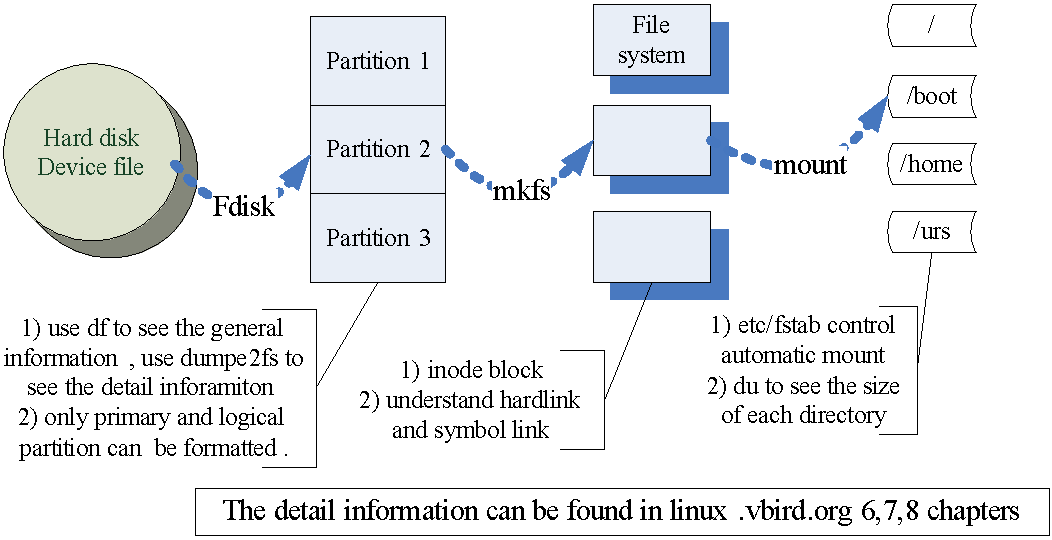
\includegraphics[scale=0.8]{pics/basic_file_system_clip}	
	\begin{itemize}
	\item You can google "where is my IP address'' to get you external IP, or use \linuxcommand{ipconfig} to know your internal IP. \linuxcommand{host} can know IP or host name from each other. Another Interesting tool is \linuxcommand{netstat} can tell you what connections are there in your computer. and \linuxcommand{traceroute} can trace the path in connection. They are some useful Internet connection tool.
	\item There are two kinds of clips, one is local clip, you only can switch data within this application, such as use Ctrl+C in kile, you only can paste in kile
	if you want to paste sth to other application, you should use shift+mouse selection and copy to xclip. middle button can paset it. In Emacs, Alt+W will copy content to global clip.
	\item *.so is shared dynamic library in linux
	\item Don't log in root, you can use \linuxcommand{sudo } follow your command
	\item Ctrl+Alt+F1\ldots F6 switch terminal. Ctrl+Alt+F7 return back to GUI
	\item install some perl programe, If you want to install in your own directory, you can add PREFIX. That will assure you have permission on it \\
  	 perl Makefile.PL  
    \begin{verbatim}
    perl Makefile.PL PREFIX=\storage\yzhao
    make
    make test
    make install
    \end{verbatim}
	\item Under linux, if you want to install programme. If there are source\_code. \\
    \begin{verbatim}
	./configure 
	make
	make install
    \end{verbatim}
	you should download from internet directly, you can't unzip it in windows. You should use tar command to unzip under linux. If you don't have root account, you can ./configure --prefix=~/program. it will compile source first, when you make install. It will copy some files to ~/program/bin or ~/program/share.
	./Configure use Makefile.in to produce Makefile. They are a set of automatic tools. You can see them in c++ web directory, but they are a little complicated, Kdevelop also use them. Just know them. OK!
	\item to make less show Chinese, \linuxcommand{export LESS=-isMrf} I don't know what it means?
	\item \linuxcommand{nice commandname \&} means that you run command friendly with other(not occupy all resources) and run it at background. Skuld may be a UNIX server!
	\item usually, virtual box think right Ctrl as default host key, it's not convinent in linux, because most of move command need right Ctrl, so you need change it.
	In window, run VBoxManage.exe setextradata global GUI/Input/HostKey 165 can change it to right Alt. Here, I need to explian, the 165, it's virtual keycode defined by
	microsoft. you can find detail in google. Now I change it to Win\_L, value is 91.
	\item There are AltGr key to input multi-language character, but I don't need it by now, according to my laptop layout, I need to change it to Alt, so I
	can use move command shortcut. and define win\_menu to Ctrl. I finish it as follow: \\
	1) use \linuxcommand{xev} get keycode, AltGr is 108 and win\_menu is 135 \\
	2) create your own .Xmodmap and write keycode 108 = Alt\_L\\
	3) in .bashrc, add some statements\\
	xmodmap -e "add Contrlo = Menu'' (this statement is very important)\\
	xmodmap -e "keycode 133 = Control\_R''\\
	\item  about keyboard shortcut, I have good idea, that is to use left Ctrl and Alt together, because you can use your thumb to press Alt and use palm to
	press Ctrl\_L,(Even in my three laptops, I also can press Ctrl\_L easily by palm).
	So a shortcut can be defined below:
	\[ \left\{ \begin{array}{cl}
	            \textrm{move} & \left\{ \begin{array}{c} \textrm{other: Ctrl\_L} \\ \textrm{emacs: Alt\_L} \end{array}  \right. \\
		    \textrm{select} & \left\{ \begin{array}{c} \textrm{other: Ctrl\_L+Shift\_L} \\ \textrm{emacs: Alt\_L+Shift\_L} \end{array}  \right. \\
	           \end{array} \right. + \left\{ \begin{array}{c}
						\textrm{left character: J} \\
						\textrm{right character: L}\\
						\textrm{upward: I}\\
						\textrm{downward: k}\\
						\textrm{left word: U}\\
						\textrm{right word: O} \\
						\textrm{begin line: H}\\
						\textrm{end line: ;}\\
						\end{array} \right.
	\]
	Delete command is below: \\
	\[ \textrm{delete} \left\{ \begin{array}{l}
	            \textrm{left character: Backspace}  \\
		    \textrm{right charcter: Ctrl\_L+N} \\
		     \textrm{left word: Ctrl\_L+Backspace}  \\
		    \textrm{right word: Ctrl\_L+M} \\
		     \textrm{line: Ctrl\_L+P}  \\
	           \end{array} \right.
	\]
	
	Question 1: why always left Ctrl? \\
	Answer: Now, if you are smart enough, you can found that there is rules inside. all the commands is left Ctrl add right hand character, becuase left Ctrl can be
	pressed by left palm and right hand is more flexible than left hand when you click the different character. \\
	Question 2: why other use Ctrl and Emacs use Alt. \\
	Answer: In common applications, Alt has been assign to trigger menu item, such as Alt+F will trigger File menu, so, I must use Ctrl. In Emacs, on the contrary,
	Ctrl has been used to trigger some common commands, so I use Alt key( and Alt is used not often as Ctrl).\\
	Question 3: How can I export my custom shortcut to other computers \\
	Answer: There are two kind of shortcut one is kate and other is kile, they store in .kde/share/apps/katepart/katepartui.rc and \linebreak[4] .kde/share/apps/kile/kileui.rc
	you can copy them and cover them in your computer. If version is different, Maybe it's a little difficult. But you can just do it within the application, it
	don't need very long time. \\
	 目前,这些键盘的定义我还没有在实践中使用过。毕竟,用箭头键太直接了,而按住ctrl在一些笔记本上不是太方便。 不过,他们依旧是一个很好的建议,以后当你使用大键盘,或者是比较密集的进行编辑工作的时候,还是非常值得尝试一下的。 
	
	\end{itemize}
\section{Environment variable}
	\begin{itemize}
	\item you should create your own bin folder under your own directory. And save your own script into it.
	Echo \$PATH will show your path setting. You can export PATH=\$PATH:/storage/yzhao/bin (add path in the end.)
	to add a new directory. Linux use : but windows use ; why windows use different?
	\item \linuxcommand{export DEPART=Sale} and \linuxcommand{DEPART=Sale ; export DEPART} they means the same. If the export statement in a script file,
	you must use \linuxcommand{Source a.sh} or \linuxcommand{. a.sh} to run the script file, then It will affect the continuous processing. source only run
	in father bash, it doesn't run in a child shell.
      \item setenv is csh command, in bash, you can use export directly.
	\item env list all the environment variables
	\item EDITOR can specify you default editor in your system.
	\item \linuxcommand{set} list all the local environment variables, that is more than env command. \linuxcommand{unset} to delete an environment variable
	\item getconf can get some system variable, such as
getconf ARG\_MAX, you can use xargs -n 50 to make command
satisfy the ARG\_MAX
	\end{itemize}

\ifx \allfiles \undefined
\end{CJK*}
\end{document}
\fi

% !Mode:: "TeX:UTF-8:Soft"
\ifx \allfiles \undefined
\documentclass[a4paper,12pt,twoside]{book}
\usepackage{CJKutf8}
\usepackage[T1]{fontenc}
\usepackage{pifont}
\usepackage{graphicx}
\usepackage{capt-of}
\usepackage{color}
\usepackage{amsmath}
\newcommand{\linuxcommand}[1]{\texttt{\textcolor{blue}{\$ #1 \Pisymbol{psy}{191}}}}
\newcommand{\op}[1]{\textcolor{blue}{-#1}}
\newcommand{\hotkey}[1]{\framebox{#1}}
\newenvironment{screen}{\sffamily}{\rmfamily}
\newcommand{\tabincell}[2]{\begin{tabular}{@{}#1@{}}#2\end{tabular}}

\begin{document}
\begin{CJK*}{UTF8}{song}
\bibliographystyle{plainnat}
\title{latex}
\author{赵岩}
\date{}\maketitle

\else
\chapter{\LaTeX}
\fi


	One important book is "A guide to latex'' \cite{Guide}, another one is "The Latex companion'' \cite{Companion}. I have the first book PDF version. and you can look up it if you have some questions. 大部分的例子和说明都于\cite{Guide}。我有这本书的电子版, 如果你在看下面的内容有什么问题的时候,你可以去参考info_center的电子版,里面有更加详细的描述。另外一个比较好的小册子就是my Latex faq,也是电子版,里面有一些比较实用的技巧。例如如何给表头加横线,如何设置图片路径,如何并排多图等。非常值得一读。
	
\section{Basic}
	\subsection{Distribution}
		\begin{tabular}{|c|c|c|c|}
		\hline 操作系统 & linux & mac & windows \\
		\hline 发布版本 & texlive & mactex( texlive) & CTEX (mictex) \\
		\hline editor & kile & texshop & winedt \\
		\hline 字体 & 没试过 & 参考\cite{MacFont} & 自动的 \\
		\hline
		\end{tabular} \\
    目前来看,对中文字体支持最好的,就应该是windows的版本了。你可以在linux或mac下编写,但是编译的时候, 推荐在windows下进行编译,因为输出的字体会比较漂亮。


	\subsection{Editor}
		常用的编辑器如下表所示:
		\begin{center}
		  \begin{tabular}{|c|c|c|c| }
		    \hline & kile & winedt & texshop \\
		    \hline 命令自动完成& 自动列表出现 & ctrl+enter & esc \\
		    \hline 插入环境& latex菜单 & insert菜单  & macro 菜单 \\
		    \hline 自动补齐& 自动 & \tabincell{c}{ \\begin\{\}\} \\ \\end\{\{ }  & \tabincell{c}{ macro\\ autocompletion.plist \\ \^\ \{\} } \\
			\hline 正反向& kdvi (ctrl+click) & yap (double click) & select (command +click) \\
			\hline outline& 自动 & 自动 & Tags (顶格写!) \\
			\hline 符号 & 工具条 & 工具条 & latex panel special characters \\
			\hline
		  \end{tabular}
		\end{center}
        winedt的工具条内容很丰富,包含了基本的常用的功能,你应该经常使用。
		\begin{itemize}
		\item Winedt 有一些编辑技巧,可以参考这个参考文献\cite{WinedtTip}。
		\item kile and winedt only support tex<-->dvi forward and backward search, and texshop support tex<-->pdf forward and backward search. So, in kile and winedt, you need to use latex to produce dvi. (Don't use pdflatex if you want to use FB search, and kile and winedt support DVI very well, and texshop didn't support dvi very well) 这个我需要解释一下,目前,我已经全部把的文档转换成了用pdflatex的格式,并没有dvi文件输出, 有没有一种方法能够支持tex->pdf的forward search功能能,如果没有,就算了。毕竟pdflatex貌似更高档一些。
		\item In Winedt, you need to add this
		\verb=\% !Mode:: "TeX:UTF-8:soft"= to the first line of tex file, it will open file with UTF8 encoding.
		\end{itemize}

	\subsubsection{kile}
		A good reference book is \cite{Kile}.\\
		\begin{description}
			\item[Forward and inverse search]:
			by now, the best supported DVI viewer is kdvi, but it has been wiped off from ubuntu, you can add it by
			\begin{verbatim}
			1. edit (in sudo of course) /etc/apt/sources.list
			2. add "deb http://archive.ubuntu.com/ubuntu/
			intrepid universe multiverse" at the last line
			3. run: sudo apt-get update
			4. run: sudo apt-get install kdvi
			\end{verbatim}
			the Forward search is ForwardDVI command. In ubuntu, It can't exchange apps automaticly, I don't know why?
			\item[Bullts]:
			It is options for some command and tabular format, you can press ctrl+alt+< to jump left and right
			\item[smart newline]:
			when you are in the item or tabular enviroment, it's useful to press shift+enter, it will insert \\item automaticly,
			\item[encode] how to change existing file encoding system, you can change it to utf8, so it will support more character.
			\item[help]
			The default Location of TeX documentation under "Settings -> Configure Kile -> Help" is set to "/usr/share/texmf/doc". It should be "/usr/share/doc/texlive-doc" as most of the TeX Documentation accessible through kile ("Help -> TeX Documentation") won't work otherwise (apart from the Documentation browser). The package texlive-doc-en has to be installed also.
			\item[error]
			if there is no error prompt, you can see file.log to see the detail information.
			\item[project]
			First, you  can create a new project, and all some files into it. The best thing for project is that you can build a tar ball directly from this project. The other is search all project files. By now, I only find these two advantages. 把一个大文章分成几个独立的章节, 这种组织方法更合理一下。这样你可以单独处理每一个独立的章节。但是,也要面临一些问题,例如, 参考文献如何组织,跨越章的交叉索引如何处理等?
		\end{description}
	

\section{beamer}
	\subsection{Tips}
	\begin{itemize}
		\item use draft option, it will not produce headlines, footlines and sidebars,\linebreak[4] \verb=\documentclass[draft]{beamer}=. Or, only compile certain frame \linebreak[4] \verb=\includeonlyframes{<frame label list>}= 用这种方法,如果你的版本比较大的时候,可以减少编译的时间。
	\end{itemize}

	\subsection{theme}
	\begin{description}
		\item[outer themes] control a slide's decorations, such as text and graphics that appear in a slide's header and footer sections. For example, \linebreak[4] \verb=\useoutertheme{shadow}= adds a 3-D shadow to some header elements.
		\item[inner themes] control a slide's inner area, such as markers/bullets for itemization lists and boxes placed around theorems. For example,\linebreak[4] \verb=\useinnertheme{rounded}= gives a rounded and 3-D look to theorem-containing boxes and itemization markers.
		\item[font themes] control font shapes and sizes of various elements of a slide show. For example, \verb=\usefonttheme{serif}= changes the document's fonts to serif. (The default is sans-serif.)
		\item[color themes] control the colors of title, frametitle, itemization bullets, and many other elements of a slide show. For example, \linebreak[4] \verb=\usecolorheme{albatross}= changes the Beamer's default colors in quite a drastic way.
	\end{description}
	you can find a good reference web here \cite{QuickStart}, it has introduced theme better, you can change color and font to see which one you like the best.
	\subsection{layout}
	There is three ways to side by side:
	\begin{itemize}
	
	\item the first one is the first is minipage
		\begin{verbatim}
		\frame{
			\begin{table}[ht]
			\begin{minipage}[b]{0.48\columnwidth}%
		    	\centering
		    	\includegraphics{filename}%
		    	% delete the above options for an exsting file
		    	\captionof{figure}{figure/table demo (Figure Caption No. 1)}
			\end{minipage}%
			\hfill%
			\begin{minipage}[b]{0.48\columnwidth}%
				\begin{tabular}{c|c}
					x     & y\\\hline
					rr    & t\\
				rrrrr & g
				\end{tabular}
				\caption{figure/table demo (Table Caption No. 1) }
			\end{minipage}
		\end{table}
		}
		\end{verbatim}

	\item the second is \verb=\subtable=
		\begin{verbatim}
			\begin{table}
			\setcounter{subtable}{0}
			 \subtable[\liuhao  开关]{
			    \begin{tabular}{|c|c|c|c|}
			           \hline 加数 &被加数&和&和\\
			           \hline 0 & 0 & 0 & 0 \\
			           \hline
			       \end{tabular}
			}
			\qquad %don't include any empty lines around here.
			\subfigure[First]{
			%\includegraphics[scale=0.4]{pics/add.png}
			}
			\end{table}
		\end{verbatim}

	\item The third one is  \verb=\columns=
		\begin{verbatim}
			\begin{columns}
			  \begin{column}{0.5\textwidth}
			    %first column.  an itemized list in it.
			    \begin{itemize}
			      \item This is an item
			      \item This is another item
			    \end{itemize}
			  \end{column}

			  \begin{column}{0.3\textwidth}
			    %second column.  a picture in it.
			    \centerline{\includegraphics[width=0.7\textwidth]{image2.png}}
			  \end{column}
			\end{columns}
		\end{verbatim}
	\end{itemize}


\section{document and article}	
	\subsection{text}
		\subsubsection{space}
		\begin{itemize}
		\item All the sequencial spaces will be regarded as one
		\item spaces at the begining are ignored
		\item end of line will be regared as one space
		\item prodce a newline but you can use \verb=\newline=, but It's still within a paragraph. That's a little different with word document. 综上,因为latex不是所见即所得,所以你需要一点技巧来使得winedt中看起来整齐; 同时,pdf中输出的也是你所希望的样子。在winedt中,不要轻易换行,你只需持续输入,如果某一行比较长, 那么就加一个空格,winedt会自动的wrap,(自动wrap有很多好处,如果换成大屏幕,他会根据屏幕宽度自动调整) 如果你需要输出单独的一行,那么就在末尾加上 \verb=\newline=或者 \verb=\\=,然后从下一行开始输入。等到完成了一个段落以后,然后加上一个\verb=\par=, 再回车,最好加一个空行。这样,就能保证winedt中相对整齐,并且和真实的输出大致一个样子。 同时,输出的格式也是我真实的希望值。每一段文字的末尾,如果后面跟着一个latex命令, 那么你就不需要在加上 \verb=\\,\par=了,否则会增加一个空行的,没有必要。如果latex命令是插入图或者是表,那么, 你就需要自己决定是否在文字后面放上换行符,如果不放,那么就是文字环绕的效果了。默认情况是文字环绕的效果。
		\item Usually, \LaTeX\ will decide the distance between word and sentence automaticly.If you want to customtize them, you can use below commands
			\begin{description}
			\item[hspace]
			\verb=\hspace{length}= will specify the horizantial distance. you can use any length unit, even a negative value.
			\verb=\hfill= will produce a rubber length.
			\verb=\quad and \qquad= will insert fixed horizontal spacing .
			\item[vspace]
			the same as \verb=\hspace=. Withing paragrah, it will increase the distance current line where command is in and next line.
			outside a paragraph, it will increase distance bewteen paragraph. if you want to change them global, see section layout
			\end{description}
		\item There is some absolute distance unit, such as cm,mm,in=(2.54cm),pt=(1 in=72.27pt). two font-specific size em=(the width of the Captial M) and ex=(the height of the letter x)
		\end{itemize}
		\subsubsection{word division}
			\begin{itemize}
			\item \LaTeX will perform this task automaticly according word-dividing algorithm. Most of time, it works well.
			\item you can use \verb=base\-line\-skip= to tell \LaTeX to make word division in this certain position.
			\item you can use \verb=\hyphenation{list}= to avoid laboriously inserting \verb=\-= verytime. you'd better make a list and put it.  but it doesn't work in \verb=\texttt{text}=. I don't know why??
			in the preamble. such as \verb=\hyphenation{man-u-script com-pu-ter ...}=
			\item Envrioment \verb=\begin{sloppypar} paragraph text \end{sloppypar}= \ does not prevent word division, but it does permit larger interword spacing without giving a warning message.
			\item if you want to avoid word division, you can use \verb=\mbox{text}= command. but it will Overfull a hbox, so don't use very often unless it is necessary.
			\end{itemize}
		\subsubsection{period}
			\begin{itemize}
			\item Uppercase follow a period is not regarded as an end sentence, if you want to change it use \verb=\@.=
			\item Lowercase follow a period is end of a sentece, if you want to change it,use space or \~{} such as \verb*=Pref. zhao or Pref.~Zhao=
			\end{itemize}
	\subsection{layout}
		\subsubsection{font}
			\begin{description}
			\item[Family]:
			\begin{minipage}{0.45\textwidth}
			 \begin{verbatim}
			\rmfamily \textrm{text}
			\ttfamily \texttt{text}
			\sffamily \textsf{text}
			\end{verbatim}
			\end{minipage}
			\begin{minipage}{0.45\textwidth}
			\textrm{abcdefghijklmn} \\
			\texttt{abcdefghijklmn} \\
			\textsf{abcdefghijklmn}
			\end{minipage}
			
			\item[Shape]:
			\begin{minipage}{0.45\textwidth}
			\begin{verbatim}
			\upshape \textup{text}
			\itshape \textit{text}
			\slahape \textsl{text}
			\scshape \textsc{text}
			\end{verbatim}
			\end{minipage}
			\begin{minipage}{0.45\textwidth}
			 \textup{abcdefghijklmn} \\
			 \textit{abcdefghijklmn}\\
			 \textsl{abcdefghijklmn}\\
			 \textsc{abcdefghijklmn}
			\end{minipage}
			\item[Series]:
			\begin{minipage}{0.45\textwidth}
			\begin{verbatim}
			\mdseries \textmd{text}
			\bfseries \textbf{text}
			\end{verbatim}
			\end{minipage}
			\begin{minipage}{0.45\textwidth}
			\textmd{abcdefghijklmn} \\
			\textbf{abcdefghijklmn}
			\end{minipage}
			\end{description}\par
			All the layout formats are based on font size. if paragraph end within the font scope, it will change the line space. such as
			\verb={\large Don't read ... \par}= and \verb={\large Don't read ... }\par = will produce output differently. \par
			{\large Don't read this this long sentence, Pay attention of distance between lines \par}
			{\large Don't read this this long sentence, Pay attention of distance between lines }\par
			here \verb=\par= is end of paragraph, it means a empty line.	
			
		\subsubsection{line distance}
			you can put \verb=\linespread{factor}= in preamble the change the distance of lines. Another better solution is: \\
			\verb=\setlength{\baselineskip}{1.5\baselineskip}=
		\subsubsection{line break}
			\verb=\\[space]=, \verb=\newline=,\verb=\linebreak[number]=, a number bwtween 0 and 4 that specifies how important a line break is. where as 4 compels a line break. the oppsite command is \verb=\nolinebreak[number]=.  if you want ot put a text together, use \verb=\mbox{text}=.
			The difference between \verb=\linebreak= and \verb=\newline= is that the current line will be fully justified.
		\subsubsection{para}
			Paragraphs are separated by blank lines, just like command \verb=\par= 你可以在\verb=\par= 后面再加一个空行,这样在winedt中更醒目一些。效果和单个\verb=\par=是一样的。
			\verb=\setlength{\parindent}{0pt}= will set indent 0 \linebreak
			\verb=\setlenght{\parskip}{1ex plus 0.5ex minus 0.2ex}= will adjust the paragraph in order to show the paragraph in a page properly. To suppress indentation for one paragraph, or to firce it where it would otherwise not occur, place \verb=\noindent= or \verb=\indent= at the beginning of the paragraph to be affected.
		\subsubsection{page break}
			\verb=\pagebreak[num]= is the equivalents of \verb=\linebreak[num]=. The opposite command is \verb=\nonpagebreak[num]=. The proper command to end a page in the middle, fill it with blank spacing, and go on to a new page is \verb=\newpage=
			\verb=\clearpage= will end the current page like \verb=\newpage= and in addition, outputs all the pending figures and tables on one or more extra pages.
		\subsubsection{page format}
			you can use \verb=\layout= to print out the basic parameter of layout. There are many kind of parameters. A simple way is to use
			\begin{verbatim}
			\usepackage{geometry}
			\geometry{a4paper,textwidth=15cm, textheight=25cm}
			\end{verbatim}
			you just need give core size, other will be adjusted automaticly.
		\subsubsection{document classification}
			%\begin{description}
			In begining, give\verb=\documentclass[option]{class}= \par
			\begin{flalign*}
			\begin{split}
			\textrm{options} \left\{ \begin{array}{l}
			\textrm{a4paper letter}
			\textrm{font size: 10pt 11pt 12pt } \\
			\textrm{onesie twoside} \\
			\textrm{onecolumn twocolumn}\\
			\textrm{openright openany}\\
			\end{array} \right.
			\end{split}&
			\end{flalign*}

			\begin{flalign*}
			\begin{split}
			\textrm{class} \left\{ \begin{array}{l}
				\textrm{book} \\ \textrm{report} \\ \textrm{article} \\ \textrm{slide}
				\end{array} \right.
			\end{split}&
			\end{flalign*}

			To simplify the structure of a book, the commands will help you to manager the page number
			\begin{verbatim}
			\frontmatter
				preface table of contents
			\mainmatter
				main body of text
			\backmatter
				bibl, index, colophon
			\end{verbatim}	
			%\end{description}

			
	\subsection{group of text}
		\subsubsection{box}
			\begin{verbatim}
				\mbox{text} and \makebox[width][pos]{text}
				\fbox{text} and \framebox[width][pos]{text}
			\end{verbatim}	
			\verb=[pos]= can have \verb=l, r, s= options. \verb=\width, \height, \depth and \totalheight= can be used to specify the \verb=[width]= such as \verb=\framebox[6\totalheight]{text}= \par

			Whole paragraphs can be put into separate vertical boxes \verb=\parbox= or with environment\verb={minipae}= you can see an example below:\par
			
			\begin{verbatim}
			\begin{minipage}[b]{4.3cm}
			 The bottom line of this minipage is aligned with the current line,
			\end{minipage}
			\hrulefill
			\begin{minipage}{3.0cm}
			 The center line of this minipage is aligned with the current line,
			\end{minipage}
			\hrulefill
			\begin{minipage}[t]{3.8cm}
			 The top line of this minipage is aligned with the current line,
			\end{minipage}
			\end{verbatim}
			will produce like this: \par

			\begin{minipage}[b]{4.3cm}
			 The bottom line of this minipage is aligned with the current line,
			\end{minipage}
			\hrulefill
			\begin{minipage}{3.0cm}
			 The center line of this minipage is aligned with the current line,
			\end{minipage}
			\hrulefill
			\begin{minipage}[t]{3.8cm}
			 The top line of this minipage is aligned with the current line,
			\end{minipage}

		\subsubsection{lists}
			\begin{verbatim}
				\begin{itemize} list text \end{itemize}
				\begin{enumerate} list text \end{enumerate}
				\begin{description} list text \end{description}
				\begin{list} list text\end{list}
			\end{verbatim}	
			如果前三个不能满足你的要求,可以用list. You can change a lot of defination in \verb=list=, a example can be found in langauge.tex file.
\section{Management}	
	\subsection{index}
			% if you write \verb=\usepackage{makeidx}, it will produce no *.idx error, WHY!!
			\begin{verbatim}
				\usepackage{makeidx}
				\makeindex
				\index
				makeindex file.idx
				\printindex
			\end{verbatim}	
	\subsection{bib}
		\begin{enumerate}
			\item define a file book.bib, you can see example in this file
			\item after \verb=\begin{document}= write \verb=\bibliographystyle{plainnat}=
			\item after \verb=\backmatter= write \verb=\bibliography{book}=
			\item in the body use \verb=\cite{Companion}=, Companion is keyword defined in linux.bib.
			\item run latex book first, produce book.aux, then run bibtex book, it will read book.aux. then run latex book.tex twice
				\begin{verbatim}
				latex book.tex
				bibtex book //产生一个book.bbl的文件。
				latex book.tex
				latex book.tex
				\end{verbatim}
			\item In mac, you can use BibDesk to manager your file.bib. In kile, you can manager your file.bib with GUI interface, (better than BibDesk and winedt)
			\end{enumerate}
        需要注意一下,如果你加入\verb=\bibliographystyle{plainnat}=这个命令,你应该运行latex或者pdflatex 命令一次,以便产生book.aux文件,因为\verb=bibtex=命令需要读取这个最新的book.aux文件。如果你还不明白, 那就按照上面的四部,从头到尾运行一遍就是。对于\verb=\bibliography{book}=命令,book.bib文件不再当前目录, 你也可以通过\verb=\bibliography{../book}=来具体指定。(本例是当前tex文件的父目录。)
		\subsection{cross reference}
			\begin{itemize}
				\item put \verb=\label{\footnote{\label{\label{} } }marker}= in section or figure or table and equation, you need give marker a description name
				\item \verb=\ref{marker}= or \verb=\pageref{marker}= to use them.
				\item \verb=marker= use hyphen to link, \verb=\labe{T-fb-result}= (It's my habit)
				\item you can use
				\begin{verbatim}
				\usepackage{capt-of}
				....
				\captionof{table or figure}{your title text}
				\label{your marker}
				\end{verbatim}
				put the \verb=\label= behind \verb=\captionof=.
	
			\end{itemize}
	\section{Picture}
		the basic command is:
		\verb!\includegraphics[key=value,...]{file_name}!
		
		\begin{description}
		\item [scale=] number; enters the number by which the figure size should be magnified over its natural size;
		\item [width=] length; specifies the width to which the figure should be scaled; if height not given, it is scaled with the same factor as the width;
		\item [height=] length; specifies the height to which the figure should be scaled; if width is not given, it is scald with the same factor as the height;
		\item [totalheight=] length; like height but specifies the height plus depth of the figure; should always be used in place of height if the figure has been rotated;
		\item [viewport=] llx lly urx ury; specifies the bounding box but relative to the lower left corner of the existing one; this is the preferred method for correcting the bounding box, or (with clip) to select only a portion of the whole figure; with pdfTEX, this option must be used rather than bb;
		\end{description}

		\begin{itemize}
		\item that is not very convient to draw a picture in \LaTeX. But it can insert eps image very easily. There are some tools in linux which can draw and export eps image. Dia can draw some diagrams very easily, because it contain some icons. If you need more beatiful effect, you can use Inkscape.
		\item
		EPS is sort of a graphic vector scripting language. \\
		PGN(GIF) is a non-lossy file format, It is very good for dirgrams, scans of drawings, or anything whose sharpness you  do want to retain, It's somethings overkill when used for photos\\
		JPG is a lossy format that compresses better than PNG at the price of some loss in the picture detail. This is usually irrelevant for photes, but many cause bad quality for diagrams, drawings, in those case use EPS or PNG. A good short description can be found \cite{Kile}, you can get this book by pressing F1 in kile. \\
		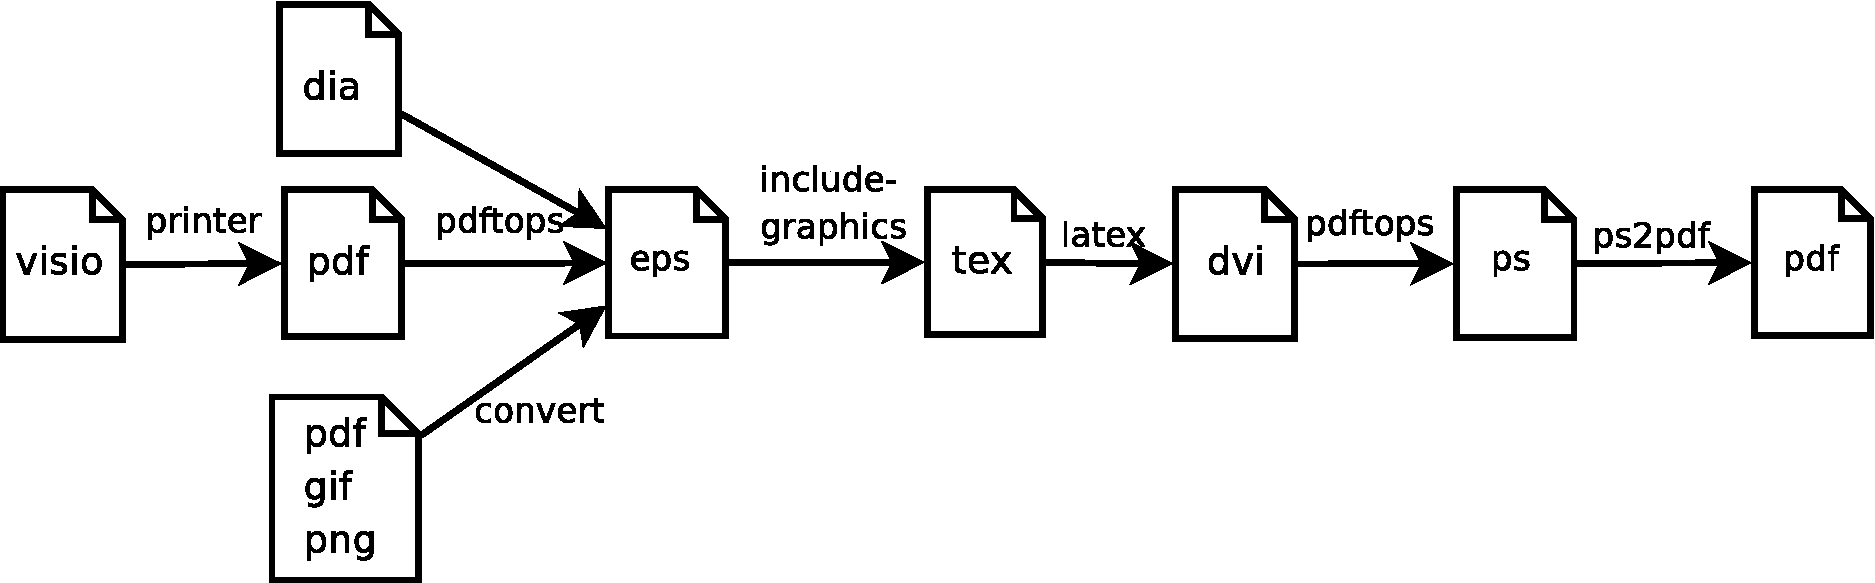
\includegraphics[scale=0.4]{pics/graphic_1}
		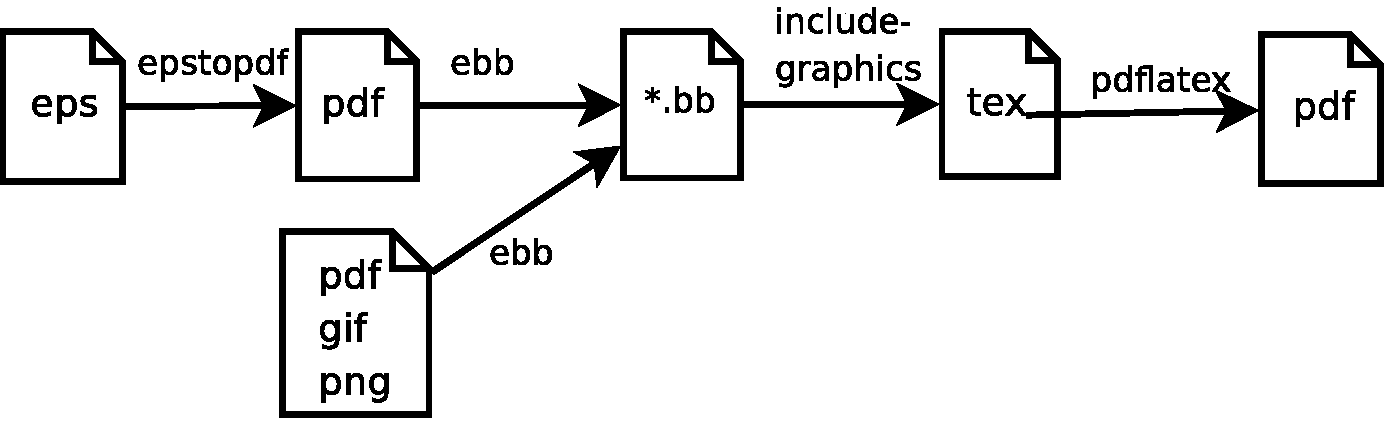
\includegraphics[scale=0.4]{pics/graphic_2} \\
		the text on the arrow is linux command and text in the frame is file format. The figure tell us that pdflatex, when used with graphics or graphicx packages, can compile correctly PNG and JPG files into DVI or PDF, but is not able to handle EPS files. Conversely, the precess of compiling with Latex to DVI and converting to PS and eventually PDF does support EPS, but doesn't supprot PNG and JPG.
		
		\item \linuxcommand{convert} is a command in ImageMagick tool package, the other commands are \linuxcommand{Identify} and \linuxcommand{combine}
		\item \linuxcommand{giftopnm myfile.gif >myfile.pnm} \linuxcommand{pnmtopng myfile.pnm myfile.png} png is new format file in internet. and pnm is intermediate format. Here I want to change gif file to png format.
		\item you can use \linuxcommand{less *.eps} to see if there is Boundbox defination.
		\item okular can view a lot of file format: pdf, ps ,dvi
		\end{itemize}
\section{math}
		\subsection{text in math}
			\begin{itemize}
			\item any space and newline has no meaning in math enoriment. you need specific command to produce space \\
				\begin{tabular}{|c|c|c|}
				\hline \verb=\,= & small space & = 3/18 of a quad \\
				\hline \verb=\:= & medium  & = 4/18 of a quad \\
				\hline \verb=\;= & large space  & = 5/18 of a quad\\
				\hline \verb=\!= & negative space  & = -3/18 of a quad\\
				\hline
				\end{tabular}
			\item What's difference between \verb=\textrm= and \verb=\mathrm= ? \\
			\verb=\[ a^\mathrm{a}_\textrm{a} \]=  will produce \[ a^\mathrm{a}_\textrm{a} \]
			can you see the diffence? the \verb=\mathrm= can change size with different postion. \verb=\textrm= is static.
			\end{itemize}
		
		\subsection{equation}
		\begin{enumerate}
		\item Simple variables are represented by italic letters, as $a b c x y z$.
		\item Vectors are written in bold face italic, as $\boldsymbol{B}$.
		\item Tensors of 2nd order and matrices may appear in a sans serif font, as
		M D I.
		\item The special numbers e, i, $\pi$, as well as the differential operator d, are to be
		written in an upright font to emphasize that they are not variables.
		\item A measurement consisting of a number plus a dimension is an indivisible
		unit, with a smaller than normal space between them, as 5.3 km and 62 kg.
		The dimension is in an upright font.
		\end{enumerate} \par

		here is two kind of formulas, text and displayed mode, the text mode exist within a line, so it don't need a equation number. (It's very easy to understand it), fractoin should be written to $a/b$ in text mode. \\	
		\[ \left\{
		\begin{array}{l}
		\textrm{text mode}	\left\{
					\begin{array}{l}
					\verb=\begin{math}...\end{math}= \\
					\verb=\(...\)= \\
					\verb=$...$=\\
					\end{array}
					\right. \vspace{2ex} \\
									
		\textrm{displayed mode}	\left\{
					\begin{array}{l}
					\textrm{number:  } \verb=\begin{equation}...\end{equation}= \\
					\textrm{no number}	\left\{
								\begin{array}{l}
								\verb=begin{displaymath}...\end{..}= \\
								\verb=\[...\]= \\
								\verb=$$...$$= \\
								\end{array}
								\right. \vspace{1ex} \\
					\end{array}
					\right.\\
		\end{array}
		\right. \]
		
		size of symbol in formula \\
		\begin{tabular}{|c|c|}
		\hline \verb=\displaystyle= & displayed formulas\\
		\hline \verb=\textstyle= & text formulas\\
		\hline \verb=\scriptstyle= & first sub-, superscript\\
		\hline \verb=\scriptscriptstyle= & later sub-, superscripts\\
		\hline
		\end{tabular} \\
		
		font will change according to the postion. \\
		\begin{tabular}{|c|c|c|c|}
		\hline active size & upper & lower & subscripts\\
		\hline D & T & T & S\\
		\hline T & S & S & S\\
		\hline S & SS & SS & SS\\
		\hline SS & SS & SS & SS\\
		\hline
		\end{tabular}

		\verb=\[ a_0 + \frac{1}{a_1 + \frac{1}{a_2 + \frac{1}{a_3 + \frac{1}{a_4}}}} \]=
		\[ a_0 + \frac{1}{a_1 + \frac{1}{a_2 + \frac{1}{a_3 + \frac{1}{a_4}}}} \]

		\begin{verbatim}
		\[ a_0 +
		\frac{1}{\displaystyle a_1 +
		\frac{1}{\displaystyle a_2 +
		\frac{1}{\displaystyle a_3 +
		\frac{1}{a_4}}}}
		\]
		\end{verbatim}
		will output
		\[ a_0 +
		\frac{1}{\displaystyle a_1 +
		\frac{1}{\displaystyle a_2 +
		\frac{1}{\displaystyle a_3 +
		\frac{1}{a_4}}}}
		\]
		array enviromnet is T \\
		D and T only difference in some symbol, such as \verb=\int \sum= \\
		\subsection{example}
			\begin{itemize}
			\item There is many kind of dots \verb=\ldots \cdots \vdots \ddots=, guess what they mean? Only \verb=\ldots= is allowed in normal text mode.
			\item text in formula should be put into \verb=\mbox{text}=
			\item \verb=\[ \oint\limits^\infty_0 \]= will produce \[ \oint\limits^\infty_0 \]
				\verb=\[ \oint^\infty_0 \]= produce \[ \oint^\infty_0 \]
				can you see the diffence with \verb=\limits=?
			\item \verb=\[ \underbrace{a + \overbrace{b + \cdots + y}^{123} + z}_{\alpha\beta\gamma} \]=
				\[ \underbrace{a + \overbrace{b + \cdots + y}^{123} + z}_{\alpha\beta\gamma} \]
				the same function include \verb=\underline \overline=
			\item  \verb!$ \vec{x} \stackrel{\mathrm{def}}{=} (x_1)$! will produce
				$ \vec{x} \stackrel{\mathrm{def}}{=} (x_1$
			\item  \verb=\begin{eqnarray}= means lines thus have the same behavior as they would in a \verb=\be gin{array} {rcl}. . . \end{array}= environment.
			\item
				\begin{verbatim}
				\begin{displaymath}
				{}^{12}_{\phantom}{1}6}\textrm{C} \qquad \textrm{versus}
				\qquad {}^{12}_6}\textrm{C}
				\end{displaymath}
				\end{verbatim}
				
				\begin{displaymath}
				{}^{12}_{\phantom{1}6}\textrm{C} \qquad \textrm{versus}
				\qquad {}^{12}_6\textrm{C}
				\end{displaymath}
			\item
				\begin{verbatim}
				\parbox{4cm}{\begin{eqnarray} \alpha &=& f(z)...\end{eqnarray}}
				\hfill \parbox{2.5cm}{\begin{eqnarray*}
				x &=& \alpha^2 - \beta^2\\ y &=& 2\alpha\beta \end{eqnarray*}}
				\hfill \begin{minipage}{4.5cm} The left-hand ... \end{minipage}
				\end{verbatim}
				
				\parbox{4cm}{\begin{eqnarray} \alpha &=& f(z)...\end{eqnarray}}
				\hfill \parbox{2.5cm}{\begin{eqnarray*}
				x &=& \alpha^2 - \beta^2\\ y &=& 2\alpha\beta \end{eqnarray*}}
				\hfill \begin{minipage}{4.5cm} The left-hand forumula is produce by parbox and minipage,you can learn from source code \end{minipage}
			\item
			\verb=\mathbf= produce bold, but upright, if you want to get italic, use \verb=\boldsymbol=
			\item
			\begin{verbatim}
				\begin{eqnarray}
				(x+y)(x-y) & = & x^2-xy+xy-y^2 \nonumber\\
				& = & x^2 - y^2 \\
				(x+y)^2
				& = & x^2 + 2xy + y^2
				\end{eqnarray}
			\end{verbatim}
			whill produce this
			\begin{eqnarray}
			(x+y)(x-y) & = & x^2-xy+xy-y^2 \nonumber\\
			& = & x^2 - y^2 \\
			(x+y)^2
			& = & x^2 + 2xy + y^2
			\end{eqnarray}

			\item \verb=\[\fbox{$\displaystyle \int^\infty_0 f(x)\,\mathrm{d}x ..$}\]=
				\[\fbox{$\displaystyle \int^\infty_0 f(x)\,\mathrm{d}x ..$}\]
			
			\item
			\verb=\substack{1st line\\2nd line\\...\\ last line}= \\
			\verb=\begin{subarray}{pos} 1st line\\2nd line\\...\\ last line \end{subarray}= \\
			\verb=\[ \sum_{\begin{subarray}{l} i\in\Lambda\\ i<j<n \end{subarray}} P(i,j) \]= produce
			\[ \sum_{\begin{subarray}{l}i\in\Lambda\\ i<j<n\end{subarray}} P(i,j) \]
			\end{itemize}
\section{table}
	\subsection{style parameters}
			\begin{description}	
			\item [\textbackslash{}tabcolsep] is half the width of the spacing that is inserted between columns in the tabular and tabular* environments;
			\item [\textbackslash{}arraycolsep] is the corresponding half intercolumn spacing for the array environment;
			\item [\textbackslash{}arrayrulewidth] is the thickness of the vertical and horizontal lines within a table;
			\item [\textbackslash{}doublerulesep] is the separation between the lines of a double rule.
			\end{description}
	
			Changes in these parameters can be made with the \verb=\setlength= command as usual. For example, to make the line thickness to be 0.5 mm, give \verb=\setlength{\arrayrulewidth}{0.5mm}= Furthermore, the parameter \verb=\arraystretch= can be used to change the distance between the rows of a table. This is a multiplying factor, with a standard value of 1. A value of 1.5 means that the inter-row spacing is increased by 50\%. A new value is set by rede?¨?ning the parameter with the command \linebreak[4] \verb=\renewcommand{\arraystretch}{factor}= \par
		\subsection{example}
			An example is listed below, It give common trip to create a table, It's enough for common useage. if you need more, you can find in the \cite{Companion}.
			\begin{verbatim}
			\begin{tabular}{|r|l||rrr|r@{:}l|r@{:}l||c|}\hline
			\multicolumn{10}{|c|}{\bfseries 1st Regional Soccer League
			Final Results 2002/03}\\ \hline
			&\itshape Club &\itshape W &\itshape T &\itshape L &
			\multicolumn{2}{c|}{\itshape Goals}
			& \multicolumn{2}{c||}{\itshape Points}
			& \itshape Remarks \\ \hline\hline
			
			1& Kingston Cowboys & 13 & 6 & 14
			& 54&45 & 32&34 & Medium Teams \\
			2 & Daysdon Bombers & 14 & 10
			& 9 & 66 & 50 & 38 & 28 & \\ \cline{1-9}
			3& Ralston Regulars & 3 & 11& 19 & 37&74 &
			17&49 & \raisebox{1.5ex}[0pt]{Demoted}\\ \hline
			\end{tabular}
			\end{verbatim}
			
			\begin{tabular}{|r|l||rrr|r@{:}l|r@{:}l||c|}\hline
			\multicolumn{10}{|c|}{ \rule[-3mm]{0mm}{8mm} \bfseries 1st Regional Soccer League
			Final Results 2002/03}\\ \hline
			&\itshape Club &\itshape W &\itshape T &\itshape L &
			\multicolumn{2}{c|}{\itshape Goals}
			& \multicolumn{2}{c||}{\itshape Points}
			& \itshape Remarks \\ \hline\hline
			
			1& Kingston Cowboys & 13 & 6 & 14 & 54&45 & 32&34 & Medium Teams \\ \hline
			2 & Daysdon Bombers & 14 & 10 & 9 & 66 & 50 & 38 & 28 & \\ \cline{1-9}
			3& Ralston Regulars & 3 & 11 & 19 & 37&74 & 17&49 & \raisebox{1.5ex}[0pt]{Demoted}\\ \hline
			\end{tabular}
			There are some notes you should know from the previous example.
			\begin{itemize}
			\item you need to understand \verb=@{:}=
			\item \verb=\rule[-3mm]{0mm}{8mm}= make the
head row higher to make it look
nice。产生一个类似于"撑子"的效果,宽度是0mm,所以是不可见的,-3mm代表把文字的下面也撑开。
			\item \verb=\raisebox= to lift the text in the last row
			\item \verb=\mulitcolumn= and \verb=cline= to make complex appearance.
			\end{itemize}

\section{User define}
	\subsection{add other .sty}
	if you can find a file.sty, copy it to tex distribution path, if It's package, maybe you need run latex command such as latex acrotex.ins. don't forget use texhash command in the end to update the search database.
	
	\subsection{counter and length}
			\[ \left\{ \begin{array}{lll}
				\textrm{counter}: \frame{\parbox{10em}{part, chapter,  section, paragraph,  page, equation, table enumi}} & \left\{ \begin{array}{ll} \textrm{change} & \left\{ \begin{array}{l}
													\verb=\setcounter= \\
													\verb=\addtocounter= \\	
													\verb=\stepcounter= \\
													\verb=\refstepcounter= \\	
												\end{array}
												\right.\\
										\textrm{user def} & \verb=\newcounter=  \\
										\textrm{custom} & \left\{ \begin{array}{l}
													 \verb=\new=\emph{counter}  \\
													\verb=\arabic= \\
													\verb=\alph= \\	
												\end{array}
												\right.
							\end{array}
						\right. \\
				\textrm{length}: \parbox{10em}{\textbackslash{}parskip, \textbackslash{}textwidth } & \left\{ \begin{array}{ll} \textrm{change} & \left\{ \begin{array}{l}
													\verb=\setlength= \\
													\verb=\addtolength= \\	
													\verb=\settowidth= \\
													\verb=\settoheight= \\
													\verb=\settodepth= \\	
												\end{array}
												\right.\\
										\textrm{user def} & \verb=\newlength=  \\
							\end{array}
						\right. \\
				\end{array}
			\right. \] \\
			\verb=\newcounter{zypage}= \\
			\verb=\setcounter{zypage}{\value{page}}= \\
			a good example is \verb=\renewcommand{\thesection}{\Alph{section}}= \\
			\begin{verbatim}
			\newlength{\zywdth}
			\newcommand{\zydefbox}[1]{\settowidth{\zywdth}{#1}}
			\newcommand{\zytextbox}[1]{\framebox[\zywdth]{#1}}
			\end{verbatim}
	\subsection{command}
		\begin{description}
		\item[Definition]:
			\begin{verbatim}
			\newcommand{\com_name}[narg][opt]{def}
			\renewcommand{\om_name}[narg][opt]{def}
			\end{verbatim}
		\item[Example]:
			\begin{verbatim}
			 \newcommand{\subvec}[3][x]{\ensuremath{#1_{#2},\ldots,#1_{#3}}}
			\end{verbatim}
			 \newcommand{\subvec}[3][x]{\ensuremath{#1_{#2},\ldots,#1_{#3}}}
			now \verb=\subvec{i}{j}= will produce
			\subvec{i}{j}. here. \verb=\ensuremath= to make
it applicable both in text and in
math.如果\verb=\subvec[a]{i}{j}=就会产生\subvec[a]{i}{j}。也就是说,如果你不提供,那么就使用默认的,如果你提供,
那么就是用你提供的。这里注意,用方括号[a]。如果没有这个optional参数,你就必须用\verb=\subver{x}{i}{j}=命令。
		\end{description}
		
	 \subsection{enviroment}.
		\begin{description}
		\item[Definition]:
			\begin{verbatim}
			\newenvironment{\env_name}[narg][opt]{beg_def}{end_def}
			\renewenvironment{\env_name}[narg][opt]{beg_def}{end_def}
			\end{verbatim}
		\item[Example]:
			\begin{verbatim}
			\newcounter{com}
			\newsavebox{\comname}
			\newenvironment{ZYcommnet}[1][zhao yan]
			{\begin{sloppypar}\noindent\stepcounter{com}\slshape
			Comment \arabic{com} \sbox{\comname}{#1}
			\begin{quote}\small\itshape}

			 {\hspace*{\fill}\usebox{\comname}\end{quote}\end{sloppypar}}
			\end{verbatim}
		
			\newcounter{com}
			\newsavebox{\comname}
			\newenvironment{ZYcomment}[1][zhao yan]
			{\begin{sloppypar}\noindent\stepcounter{com}\slshape
			Comment \arabic{com} \sbox{\comname}{#1}
			\begin{quote}\small\itshape}
			 {\hspace*{\fill}\usebox{\comname}\end{quote}\end{sloppypar}}

        \begin{verbatim}
          \begin{ZYcomment}[ZhaoYan]
			Any thing can be finished by you hard work...
			\end{ZYcomment}
        \end{verbatim}
		will produce: \\	
			\begin{ZYcomment}[ZhaoYan]
			Any thing can be finished by you hard work...
			\end{ZYcomment}
		\end{description}
		


\ifx \allfiles \undefined
\bibliography{../book}
\end{CJK*}
\end{document}
\fi



\backmatter
\bibliography{book}
\end{CJK*}
\end{document}
